\documentclass[12pt,a4paper]{report}
\usepackage[utf8]{inputenc}
\usepackage[T5]{fontenc}
\usepackage[english]{babel}
\selectlanguage{english}
\AtBeginDocument{%
  \renewcommand{\chaptername}{Chapter}%
  \renewcommand{\contentsname}{Table of Contents}%
  \renewcommand{\listfigurename}{List of Figures}%
  \renewcommand{\listtablename}{List of Tables}%
  \renewcommand{\bibname}{References}%
  \renewcommand{\figurename}{Figure}%
  \renewcommand{\tablename}{Table}%
}
\usepackage{graphicx}
\usepackage[table]{xcolor}
\usepackage{geometry}
\setlength{\parindent}{0pt}
\setlength{\parskip}{6pt}
\usepackage{amsmath}
\usepackage{amssymb}
\usepackage{hyperref}
\usepackage{amsmath}
\usepackage{booktabs}
\usepackage{longtable}
\usepackage{array}
\usepackage{titlesec}
\usepackage{float}
\usepackage{tikz}
\usetikzlibrary{positioning, arrows.meta}
\titleformat{\subsection}{\normalfont\normalsize\bfseries}{\thesubsection}{1em}{}

\geometry{
    top=2.5cm,
    bottom=2.5cm,
    left=3cm,
    right=2.5cm
}

\begin{document}

% COVER PAGE
\thispagestyle{empty}

\begin{center}

% USTH Logo

\includegraphics[width=3cm]{images/usth_logo.png}

\vspace{0.5cm}

% University Name
{\Large\textbf{University of Science and Technology of Hanoi}}

\vspace{0.3cm}

% Report Type
{\large Final Thesis}

\vspace{1.5cm}

% Horizontal rule
\rule{\textwidth}{1.5pt}

\vspace{0.5cm}

% Title
{\LARGE\textbf{Optimizing Shape Diameter Function\\[0.3cm] using High Performance Computing}}

\vspace{0.5cm}

% Horizontal rule
\rule{\textwidth}{1.5pt}

\vspace{2cm}

% Authors
{\large\textit{Authors:}}

\vspace{0.3cm}

{\large Nguyễn Đức Đạt}

\vspace{1.5cm}

% Supervisors
{\large\textit{Supervised by:}}

\vspace{0.3cm}

{\large Dr.\ Nguyễn Hoàng Hà\\[0.2cm]
Prof.\ Lilian Aveneau}

\end{center}

\newpage
\thispagestyle{empty}
\addtocounter{page}{-1}


% CHAPTER 1: INTRODUCTION
\chapter{Introduction}

Here, we'll dive into the basics of the Shape Diameter Function (SDF), which is a really fancy way of figuring out how thick or thin a 3D object is. We'll explore what the SDF is, why we care about it, how others have tried to compute it using GPUs, and what we're going to achieve in this thesis.

\section{Context}

But what exactly is the Shape Diameter Function? Introduced by Shapira et al.\ \cite{shapira2008}, you can think of the SDF as a tool that measures the "thickness" of a 3D model at any given point on its surface. Imagine you are standing on the surface of a 3D model at a specific point $p$. If you look straight down into the object (along the negative normal $-\vec{\mathbf{n}}$), how deep is it before you pop out the other side? That depth is essentially what the SDF measures!

However, just measuring a single straight line can give us wonky results if the object is bumpy inside. To solve this, we don't just shoot one straight line. Instead, we shoot a whole "cone" of rays inward from point $p$. We measure how far each ray travels before hitting the opposite wall, and then we calculate the average of all those distances:

\begin{equation}
    \text{SDF}(p) = \frac{\sum_{i=1}^{R} d_i \cdot w_i}{\sum_{i=1}^{R} w_i}
\end{equation}

\begin{figure}[H]
\centering
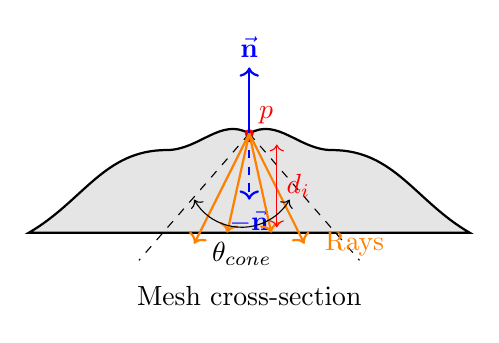
\begin{tikzpicture}[scale=0.7]
    % Draw mesh surface (cross-section)
    \draw[thick, fill=gray!20] (-4,0) to[out=30,in=180] (-1.5,1.5) to[out=0,in=150] (0,1.8) to[out=30,in=180] (1.5,1.5) to[out=0,in=150] (4,0) -- cycle;
    
    % Point p on surface
    \filldraw[red] (0,1.8) circle (2pt) node[above right] {$p$};
    
    % Normal vector (outward)
    \draw[blue, thick, ->] (0,1.8) -- (0,3.0) node[above] {$\vec{\mathbf{n}}$};
    
    % Inverted normal (inward)
    \draw[blue, thick, ->, dashed] (0,1.8) -- (0,0.6) node[below] {$-\vec{\mathbf{n}}$};
    
    % Cone boundary lines (dashed)
    \draw[dashed] (0,1.8) -- (-2.0,-0.5);
    \draw[dashed] (0,1.8) -- (2.0,-0.5);
    
    % Cone of rays (solid orange)
    \draw[orange, thick, ->] (0,1.8) -- (-1.0,-0.2);
    \draw[orange, thick, ->] (0,1.8) -- (-0.4,0.0);
    \draw[orange, thick, ->] (0,1.8) -- (0.4,0.0);
    \draw[orange, thick, ->] (0,1.8) -- (1.0,-0.2);
    
    % Distance annotation (along one ray)
    \draw[red, <->] (0.5,1.6) -- (0.5,0.1) node[midway, right] {$d_i$};
    
    % Cone angle arc
    \draw[<->] (-1.0,0.6) arc[start angle=210,end angle=330,radius=1.0] node[midway, below=2pt] {$\theta_{cone}$};
    
    % Labels
    \node[below] at (0,-0.8) {Mesh cross-section};
    \node[orange, right] at (1.2,-0.2) {Rays};
\end{tikzpicture}
\caption{Illustration of the SDF computation.}
\label{fig:sdf_concept}
\end{figure}

Figure~\ref{fig:sdf_concept} shows a visual breakdown of this process. A cone of rays is shot inward from point $p$. Each ray travels until it hits the opposite wall, recording its travel distance $d_i$. But are all rays treated equally? Nope! Rays shooting straight down the middle are usually more accurate than rays shooting out at wide angles ($\theta_i$). Because of this, we give the straighter rays a higher "weight" ($w_i$). The final SDF value is just the average of these weighted distances (typically using $R = 64$ rays).

As you might guess, a thick area (like a person's torso) will have very long ray distances, resulting in a large SDF value. However, a thin area (like a finger or an ear) will have very short ray distances, resulting in a small SDF value. Because this measurement relies purely on the object's volume, you can spin the object around or bend its arms and legs, and the thickness values won't change!

\begin{figure}[ht]
\centering
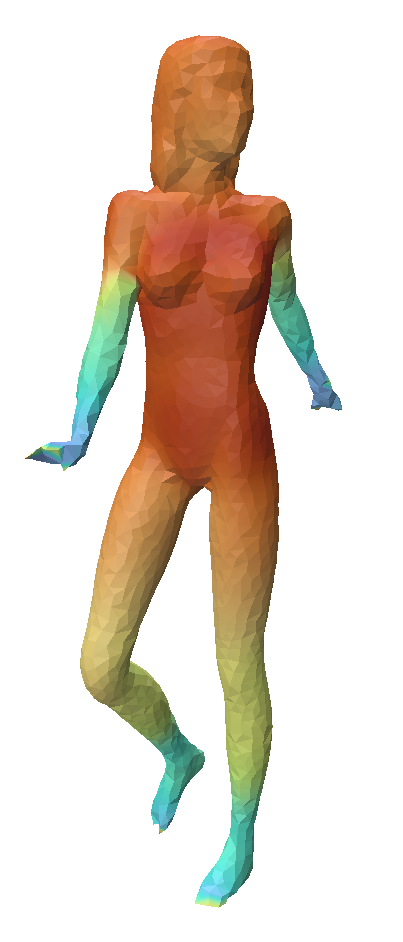
\includegraphics[width=0.45\textwidth]{images/Chapter3/Introduction/Torso.PNG}
\caption{A 3D model of a human torso SDF value heatmap.}
\label{fig:torso}
\end{figure}

Figure~\ref{fig:torso} shows a 3D model of a human torso. The SDF values are highest in the chest and abdomen regions, where the volume is thickest, and decrease toward the neck and shoulders.

\section{Why SDF: Role in 3D Object Analysis}

But why do we care about how thick a 3D model is? It turns out that knowing an object's thickness is incredibly useful for computers! For example, it helps with mesh segmentation (cutting a 3D model into logical pieces, like separating an arm from a body because the wrist is thinner), skeletonization (finding the "bones" inside a 3D character by tracing the thickest parts), and even character animation (figuring out how a 3D character should bend and move naturally).

However, there is a catch. Figuring out the thickness for millions of points on a highly detailed 3D model takes a massive amount of math. Doing this on a standard computer processor (CPU) is agonizingly slow. This bottleneck led researchers to start moving the math over to graphics cards (GPUs), which are amazing at doing thousands of tiny math problems at the exact same time.

\section{Survey of Existing Work}

Several approaches have been developed for computing the SDF on the GPU.

\subsection{PyMeshLab GPU (VCGlib)}

PyMeshLab uses a trick with computer graphics (OpenGL) called the ``spawning camera'' technique \cite{vcglib}. Think of it like placing virtual security cameras all around the 3D object. Each camera takes a picture of how deep the object looks from its specific angle. By blending all these pictures together, it figures out the overall thickness!

But there's a problem with this. Setting up all these virtual cameras and combining their pictures requires a lot of setup time. Because of this heavy setup, even tiny, simple 3D models still take at least 0.3 seconds to process.

\subsection{Kamenick\'{y} -- OpenCL Parallelization}

Kamenick\'{y} \cite{kamenicky2014} tried a different approach using OpenCL (a tool that lets programs run on different types of graphics cards). They proved that if you shoot the rays in parallel using the GPU, you get a massive speed boost over traditional CPU methods.

However, OpenCL is a bit of a ``jack of all trades.'' It works on many devices, but it misses out on the specialized, ultra-fast ray tracing hardware (like RT Cores) built into modern NVIDIA cards.

\subsection{Fast and Robust Shape Diameter Function}

Chen et al.\ \cite{chen2018} realized that shooting dozens of rays from every single point was slow and sensitive to bumpy, noisy surfaces. So, they wrapped the whole 3D model in a smooth virtual bubble (an ``offset surface''). By measuring from this smooth bubble instead of the bumpy surface itself, they only needed to shoot a single ray per point! This clever trick made the process about 10 times faster and handled broken or noisy 3D models perfectly.

\section{Objective}

So, where do we fit into all of this? The main goal of this thesis is to build the ultimate, high-speed SDF calculator using modern High Performance Computing. Specifically, we aim to build a super-fast pipeline using NVIDIA OptiX to take full advantage of specialized ray tracing hardware (RT Cores), pit our new OptiX approach against the existing PyMeshLab camera-trick method to see who wins in speed and accuracy, and prove that using dedicated ray tracing hardware is the best way to compute 3D thickness.

Now that we know what we're building and why, the next chapter will introduce the awesome tools we'll be using to make it happen (like NVIDIA OptiX and CUDA).


% CHAPTER 2: MATERIALS AND TECHNOLOGIES
\chapter{Materials and Technologies}

This chapter introduces the core technologies used to implement the high-performance SDF computation pipeline. We describe the CUDA parallel computing platform, the NVIDIA OptiX ray tracing framework, and the dataset of 3D models used for evaluation.

\section{CUDA}

CUDA (Compute Unified Device Architecture) \cite{cuda} is NVIDIA's parallel computing platform. In this project, CUDA is used for kernel execution (launching massively parallel kernels for normal computation, SDF normalization, and anisotropic smoothing), memory management (allocating and managing GPU memory for mesh data, intermediate results, and output buffers), and the CUB library (using CUB's device-wide primitives for radix sort and unique operations when building the mesh adjacency graph in CSR format).

The key CUDA kernels implemented in this project include \texttt{GPUComputeBoundingBox} (computes the mesh bounding box using atomic min/max operations), \texttt{GPUComputeSDFMinMax} and \texttt{GPUApplySDFNormalization} (min-max normalization with logarithmic compression), \texttt{GPUGenerateEdges} and \texttt{GPUExtractCSR} (constructs the Compressed Sparse Row adjacency graph), and \texttt{AnisotropicSmoothingKernel} (bilateral smoothing kernel operating on the mesh graph).

\section{NVIDIA OptiX}

NVIDIA OptiX \cite{optix} is a high-level framework for ray tracing on NVIDIA GPUs. It provides hardware-accelerated ray tracing by leveraging NVIDIA RT Cores (available on Turing, Ampere, and newer architectures) to accelerate ray-triangle intersection tests in hardware. It automatically builds and maintains Bounding Volume Hierarchy (BVH) acceleration structures, enabling $O(\log F)$ ray-triangle intersection queries. The framework supports programmable shaders, allowing custom ray generation, miss, and closest-hit programs written in CUDA. It also enables zero-copy computation, where data remains on the GPU throughout the pipeline, eliminating host-device transfer overhead.

\begin{figure}[ht]
\centering
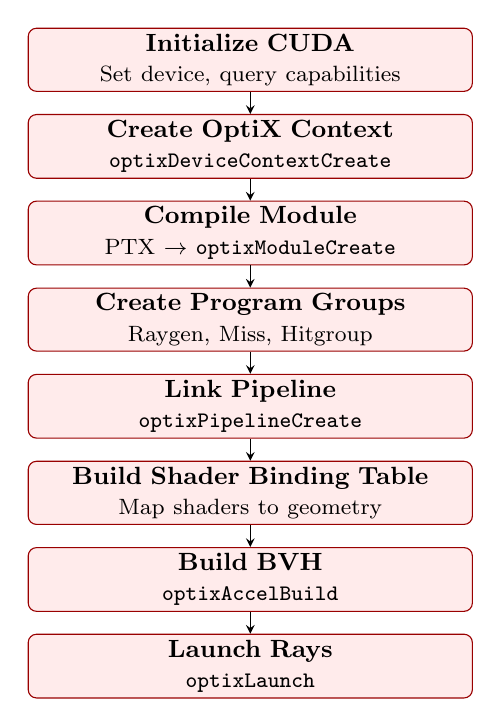
\begin{tikzpicture}[
    >=stealth,
    box/.style={
        rectangle,
        rounded corners=3pt,
        draw=red!60!black,
        fill=red!8,
        text width=5.5cm,
        minimum height=0.7cm,
        align=center,
        font=\small,
        inner sep=2pt
    },
    arr/.style={
        ->,
        -{stealth[length=2.5mm,width=2mm]}
    }
]

\node[box] (cuda) at (0, 0) {\textbf{Initialize CUDA}\\{\footnotesize Set device, query capabilities}};
\node[box] (ctx) at (0, -1.1) {\textbf{Create OptiX Context}\\{\footnotesize \texttt{optixDeviceContextCreate}}};
\node[box] (module) at (0, -2.2) {\textbf{Compile Module}\\{\footnotesize PTX $\to$ \texttt{optixModuleCreate}}};
\node[box] (prog) at (0, -3.3) {\textbf{Create Program Groups}\\{\footnotesize Raygen, Miss, Hitgroup}};
\node[box] (pipe) at (0, -4.4) {\textbf{Link Pipeline}\\{\footnotesize \texttt{optixPipelineCreate}}};
\node[box] (sbt) at (0, -5.5) {\textbf{Build Shader Binding Table}\\{\footnotesize Map shaders to geometry}};
\node[box] (bvh) at (0, -6.6) {\textbf{Build BVH}\\{\footnotesize \texttt{optixAccelBuild}}};
\node[box] (launch) at (0, -7.7) {\textbf{Launch Rays}\\{\footnotesize \texttt{optixLaunch}}};

\draw[arr] (cuda) -- (ctx);
\draw[arr] (ctx) -- (module);
\draw[arr] (module) -- (prog);
\draw[arr] (prog) -- (pipe);
\draw[arr] (pipe) -- (sbt);
\draw[arr] (sbt) -- (bvh);
\draw[arr] (bvh) -- (launch);

\end{tikzpicture}
\caption{Formal OptiX initialization sequence. Each step must be completed in order before rays can be traced.}
\label{fig:optix_init}
\end{figure}

The OptiX pipeline for SDF computation consists of module creation (compiling CUDA shader code to PTX and creating an OptiX module), program groups (defining ray generation, miss, and hit group programs), pipeline linking (connecting program groups into a traceable pipeline), Shader Binding Table (SBT) configuration (mapping shaders to geometry), BVH construction (building the acceleration structure from triangle mesh data), and launch (executing the ray tracing kernel across all vertices).

\section{Technology Selection}

The choice of OptiX + CUDA over alternative technologies was driven by several factors summarized in Table~\ref{tab:tech_compare}.

\begin{table}[h]
\centering
\begin{tabular}{@{}lll@{}}
\toprule
\textbf{Criterion} & \textbf{OptiX + CUDA} & \textbf{OpenGL (VCGlib)} \\
\midrule
Ray tracing & Hardware RT Cores & Software rasterization \\
BVH traversal & $O(\log F)$ hardware & None (depth peeling) \\
GPU requirement & NVIDIA RTX & Any GPU with OpenGL 3.3+ \\
Post-processing & Full GPU pipeline & None \\
Parallelism model & Per-vertex & Per-direction \\
\bottomrule
\end{tabular}
\caption{Comparison of OptiX vs.\ OpenGL approaches}
\label{tab:tech_compare}
\end{table}

As shown in Table~\ref{tab:tech_compare}, the OptiX + CUDA approach provides hardware-accelerated ray tracing through dedicated RT Cores, enabling $O(\log F)$ BVH traversal directly in hardware. The OpenGL approach relies on software rasterization with depth peeling and requires multiple camera directions to approximate thickness from all sides. OptiX's per-vertex parallelism maps naturally to the SDF computation (each vertex independently shoots rays), while OpenGL's per-direction parallelism requires $N$ separate draw calls with accumulated blending. The post-processing pipeline (log normalization and bilateral smoothing) runs entirely on the GPU in the OptiX approach, whereas the OpenGL approach has no built-in post-processing support.

\section{Dataset}

The evaluation dataset consists of 13 triangular mesh models in OBJ format, stored in the \texttt{Model/} directory. These models vary in complexity and size as shown in Table~\ref{tab:dataset}.

\begin{table}[h]
\centering
\begin{tabular}{@{}lrr@{}}
\toprule
\textbf{Model} & \textbf{Vertices} & \textbf{Description} \\
\midrule
360.obj & 2,200 & Simple object \\
9.obj & 2,639 & Simple object \\
400.obj & 3,703 & Medium complexity \\
76.obj & 5,923 & Medium complexity \\
181.obj & 7,242 & Medium complexity \\
118.obj & 9,153 & High complexity \\
368.obj & 11,202 & High complexity \\
112.obj & 13,628 & High complexity \\
369.obj & 13,606 & High complexity \\
158.obj & 14,587 & High complexity \\
371.obj & 14,599 & High complexity \\
Leaf.obj & 24,866 & Highest complexity \\
\bottomrule
\end{tabular}
\caption{Dataset models and vertex counts}
\label{tab:dataset}
\end{table}

As shown in Table~\ref{tab:dataset}, the dataset spans a wide range of mesh complexities, from simple objects like 360.obj with 2,200 vertices to highly detailed models like Leaf.obj with 24,866 vertices. This diversity ensures that the benchmark results are representative across different scales of geometric detail. The models are triangular meshes in OBJ format, which is the standard input format for the SDF computation pipeline. The vertex counts are used in Chapter 4 to analyze how computation time scales with model complexity.

The models were selected to cover a range of vertex counts (from 2,200 to 24,866) to evaluate how each implementation scales with mesh complexity.


% CHAPTER 3: METHODOLOGY
\chapter{Methodology}

Welcome to the core of the project! In this chapter, we're going to break down the entire process (or "pipeline") of how we actually compute the thickness of a 3D model using NVIDIA OptiX. We will walk through the whole journey, from the moment we load a 3D model into the computer to the moment we get our final, smoothed-out thickness values. The whole process has four main phases: reading the file, figuring out which way the surface is facing, shooting the rays, and cleaning up the final math. Figure~\ref{fig:pipeline} shows the complete roadmap.

\begin{figure}[ht]
\centering
\makebox[\textwidth][c]{\resizebox{1.3\textwidth}{!}{%
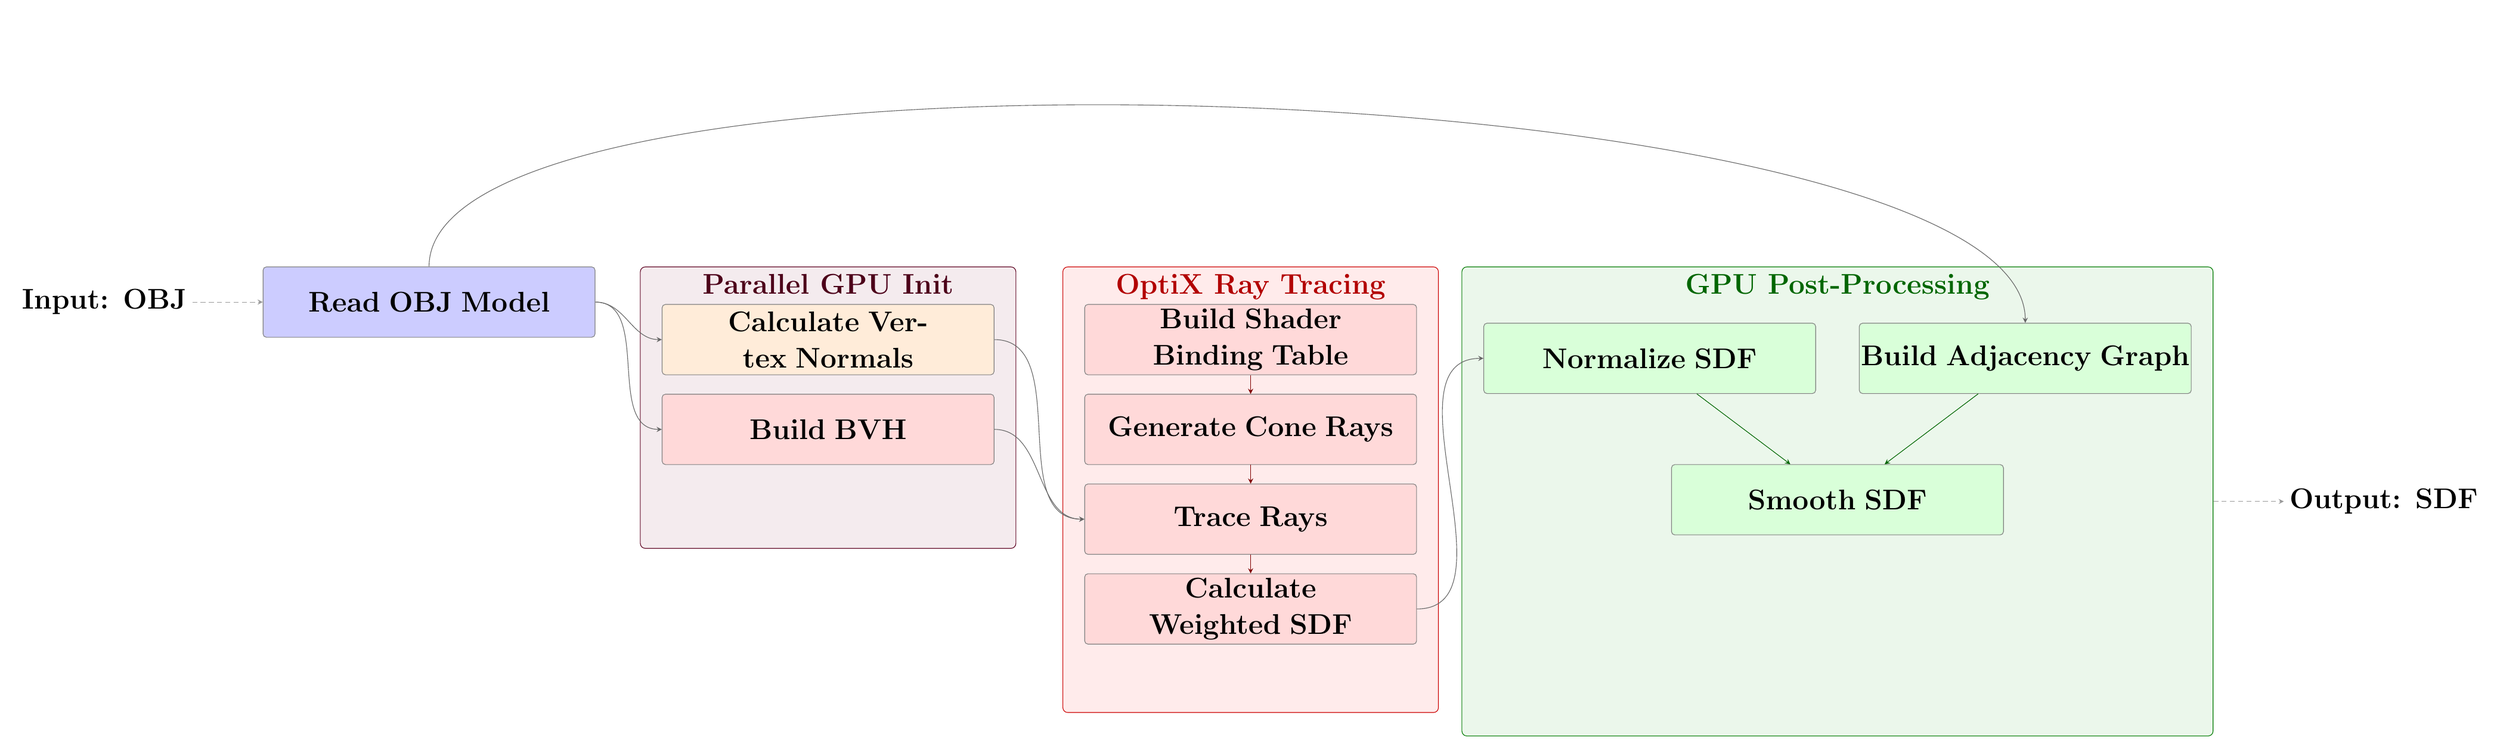
\begin{tikzpicture}[
    >=stealth,
    stage/.style={
        rectangle,
        rounded corners=2pt,
        draw=black!50,
        fill=#1,
        text width=7.0cm,
        minimum height=1.5cm,
        align=center,
        font=\fontsize{18}{22}\selectfont,
        inner sep=1pt
    },
    domain/.style={
        rectangle,
        rounded corners=3pt,
        draw=#1!80!black,
        fill=#1!8,
        line width=0.4pt,
        inner sep=4pt
    },
    arr/.style={
        ->,
        -{stealth[length=1.5mm,width=1.2mm]}
    }
]

% --- CPU: just the stage box, no outer domain box ---
\node[stage=blue!20, anchor=north] (load) at (0, 0) {\bfseries Read OBJ Model};

% --- Parallel GPU Initialization Domain (with outer box) ---
\node[domain=purple!60!black, minimum width=8.0cm, minimum height=6.0cm, anchor=north] (parallel_box) at (8.5cm, 0) {};
\node[anchor=north, font=\fontsize{18}{22}\selectfont\bfseries, text=purple!40!black] at ([yshift=-1pt]parallel_box.north) {Parallel GPU Init};

\node[stage=orange!15, anchor=north] (normal) at ([yshift=-0.8cm]parallel_box.north) {\bfseries Calculate Vertex Normals};
\node[stage=red!15, anchor=north] (bvh) at ([yshift=-0.4cm]normal.south) {\bfseries Build BVH};

% --- OptiX Domain (with outer box) ---
\node[domain=red, minimum width=8.0cm, minimum height=9.5cm, anchor=north] (optix_box) at (17.5cm, 0) {};
\node[anchor=north, font=\fontsize{18}{22}\selectfont\bfseries, text=red!70!black, align=center] at ([yshift=-1pt]optix_box.north) {OptiX Ray Tracing \\ Engine};

\node[stage=red!15, anchor=north] (sbt) at ([yshift=-0.8cm]optix_box.north) {\bfseries Build Shader Binding Table};
\node[stage=red!15, anchor=north] (raygen) at ([yshift=-0.4cm]sbt.south) {\bfseries Generate Cone Rays};
\node[stage=red!15, anchor=north] (trace) at ([yshift=-0.4cm]raygen.south) {\bfseries Trace Rays};
\node[stage=red!15, anchor=north] (rawsdf) at ([yshift=-0.4cm]trace.south) {\bfseries Calculate Weighted SDF};

\draw[arr, red!50!black] (sbt) -- (raygen);
\draw[arr, red!50!black] (raygen) -- (trace);
\draw[arr, red!50!black] (trace) -- (rawsdf);

% --- GPU Post-Processing Domain (with outer box) ---
\node[domain=green!60!black, minimum width=16.0cm, minimum height=10.0cm, anchor=north] (post_box) at (30cm, 0) {};
\node[anchor=north, font=\fontsize{18}{22}\selectfont\bfseries, text=green!40!black] at ([yshift=-1pt]post_box.north) {GPU Post-Processing};

\node[stage=green!15, anchor=north] (norm) at ([xshift=-4.0cm, yshift=-1.2cm]post_box.north) {\bfseries Normalize SDF};
\node[stage=green!15, anchor=north] (csr) at ([xshift=4.0cm, yshift=-1.2cm]post_box.north) {\bfseries Build Adjacency Graph};
\node[stage=green!15, anchor=north] (smooth) at ([yshift=-1.5cm]norm.south -| post_box.center) {\bfseries Smooth SDF};

\draw[arr, green!40!black] (norm) -- (smooth);
\draw[arr, green!40!black] (csr) -- (smooth);

% --- Inter-domain arrows ---
\draw[arr, black!60] (load.east) to[out=0, in=180] (normal.west);
\draw[arr, black!60] (load.east) to[out=0, in=180] (bvh.west);
\draw[arr, black!60] (normal.east) to[out=0, in=180] (trace.west);
\draw[arr, black!60] (bvh.east) to[out=0, in=180] (trace.west);
\draw[arr, black!60] (rawsdf.east) to[out=0, in=180] (norm.west);
\draw[arr, black!60] (load.north) to[out=90, in=90, looseness=0.4] (csr.north);

% --- Input/Output ---
\node[font=\fontsize{18}{22}\selectfont\bfseries, left=1.5cm of load.west, anchor=east] (input) {Input: OBJ};
\draw[arr, densely dashed, black!40] (input) -- (load.west);

\node[font=\fontsize{18}{22}\selectfont\bfseries, right=1.5cm of post_box.east, anchor=west] (output) {Output: SDF};
\draw[arr, densely dashed, black!40] (post_box.east) -- (output);

\end{tikzpicture}%
}}
\caption{Overall OptiX SDF computation pipeline with parallel execution.}
\label{fig:pipeline}
\end{figure}

As you can see in Figure~\ref{fig:pipeline}, the workflow has been upgraded to a highly parallel architecture. It starts by loading the 3D model on the CPU (the blue box). To maximize hardware utilization, the system then executes two heavy initialization tasks simultaneously using CUDA streams: calculating the vertex normals on the GPU and building the OptiX Bounding Volume Hierarchy (BVH) structure (the purple box). Once both are complete, it hands the physics simulation over to the OptiX ray tracing engine (the red box), and finally cleans up the data with a GPU post-processing stage (the green box). This parallelization significantly reduces the pipeline's startup time!

\section{Read OBJ Model}

Triangles form every 3D model. The triangle data is saved in the .obj file. First, it stores the position of every vertex that forms the 3D model. Secondly, it stores the links between the vertices that define the triangular faces.

\begin{figure}[H]
\centering
\begin{minipage}{0.48\textwidth}
\centering
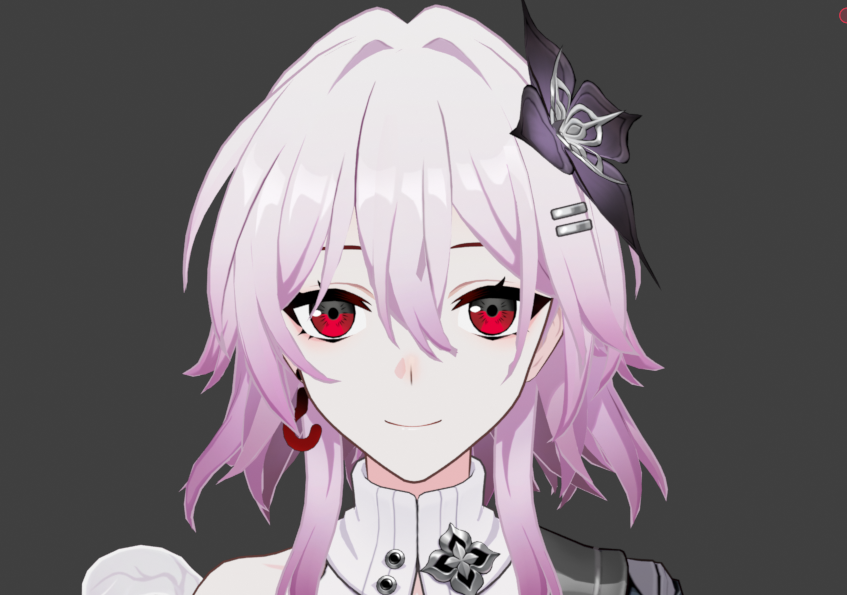
\includegraphics[width=\textwidth]{images/Chapter3/3.1/Figure 3D model example.PNG}
\caption*{\large (a) A complex 3D model rendered with solid shading.}
\end{minipage}
\hfill
\begin{minipage}{0.48\textwidth}
\centering
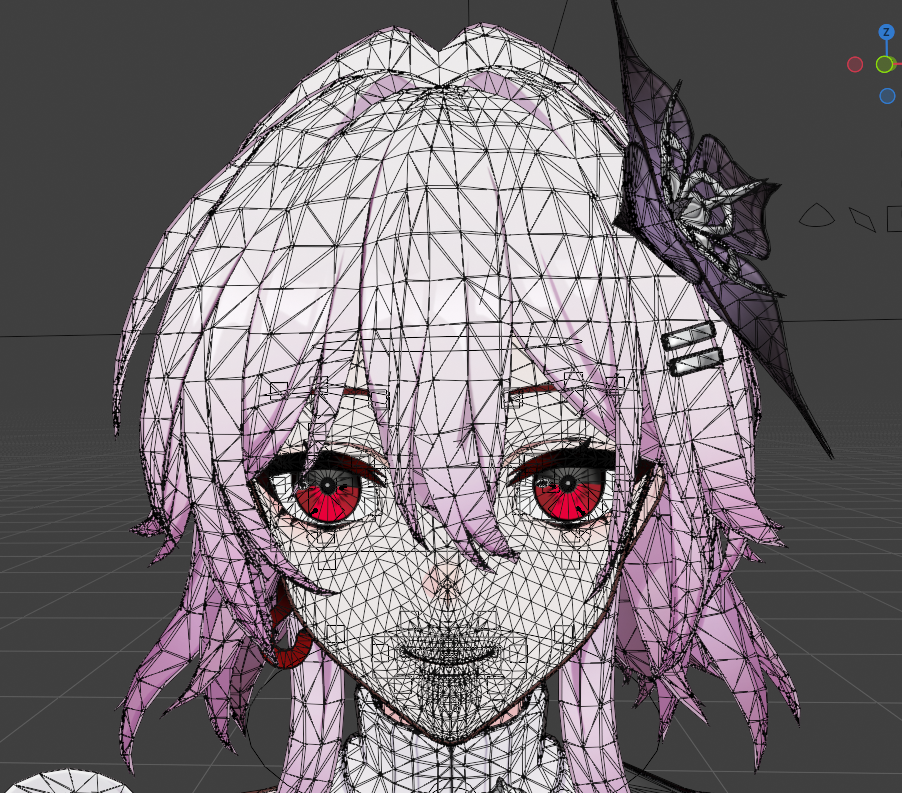
\includegraphics[width=\textwidth]{images/Chapter3/3.1/Figure 3D model wireframe (triangles).PNG}
\caption*{\large (b) The same model showing the triangular mesh wireframe structure.}
\end{minipage}
\caption[A 3D model (a) and its wireframe representation (b) composed of triangles.]{A 3D model (a) and its wireframe representation (b) composed of triangles.}
\label{fig:3d_model_example}
\end{figure}

Figure~\ref{fig:3d_model_example} shows that complex 3D shapes are fundamentally constructed from a dense network of interconnected triangles. Every 3D surface is approximated by a collection of triangular faces, where each triangle is defined by three vertices and their connectivity.

\begin{figure}[H]
\centering
\begin{Verbatim}[ fontsize=\small, frame=single, framesep=3mm, numbers=left, numbersep=5pt]
# cube.obj - Sample OBJ file
# Vertex positions (x y z)
v  1.0  1.0  0.0  # (1st vertex)
v  1.0 -1.0  0.0  # (2nd vertex)
v -1.0 -1.0  0.0  # (3rd vertex)
v -1.0  1.0  0.0  # (4th vertex)
v  1.0  1.0  1.0
v  1.0 -1.0  1.0
v -1.0 -1.0  1.0
v -1.0  1.0  1.0
# Faces (vertex indices, 1-based)
f 1 2 3  # <- connect vertex 1, vertex 2, vertex 3 to form a triangle
f 1 3 4  # <- connect vertex 1, vertex 3, vertex 4 to form a triangle
# 2 triangles combine to form a square face (vertices 1, 2, 3, 4)
f 5 6 7
f 5 7 8
f 1 2 6
f 1 6 5
f 3 4 8
f 3 8 7
f 1 4 8
f 1 8 5
f 2 3 7
f 2 7 6
\end{Verbatim}
\caption{Structure of a sample Cube 3D object saving in the textlike .OBJ file.}
\label{fig:obj_structure}
\end{figure}

Figure~\ref{fig:obj_structure} shows the structure of a sample OBJ file. The file uses a simple text format where lines starting with \texttt{v} define points in 3D space (called vertices), and lines starting with \texttt{f} define flat faces by connecting three of those points. Popular graphics APIs like Vulkan or DirectX use three points instead of two for the connection between vertices because every flat surface has two sides: a front and a back. To optimize rendering, the GPU only draws the visible front faces and hides the back faces. However, the graphics API does not automatically know which side is the front, so you must define it manually by the order in which you connect the points (known as winding order). For example, if you define a face with vertices \texttt{f 1 2 3}, the API connects the points in a counter-clockwise direction, which manually defines it as the front face. If you replace it with \texttt{f 1 3 2}, it swaps the front face to the opposite side.

The program starts by reading the 3D model data from the OBJ file. A component called the \texttt{Model} class goes through the text and extracts two main lists: the points ($x, y, z$ coordinates) and the faces (which three points form a triangle). Because OBJ files start counting items from 1, the program subtracts 1 from the face numbers so they start at 0, which is how the graphics card (GPU) prefers to count.

These lists are then packed into two simple data matrices for the GPU. The first is a vertex matrix where each row holds the coordinates of a single point. The second is a face matrix where each row holds the three point IDs that make up a triangle. These matrices are sent to the GPU memory once and reused for all the calculations that come next. For example, using the data from the sample Cube OBJ file above, the resulting GPU matrices would look like this:

\begin{equation}
\mathbf{V} = \begin{bmatrix}
1.0 & 1.0 & 0.0 \\
1.0 & -1.0 & 0.0 \\
-1.0 & -1.0 & 0.0 \\
\vdots & \vdots & \vdots
\end{bmatrix}, \quad
\mathbf{F} = \begin{bmatrix}
0 & 1 & 2 \\
0 & 2 & 3 \\
4 & 5 & 6 \\
\vdots & \vdots & \vdots
\end{bmatrix}
\end{equation}

The \texttt{Model::ReadFromObjFile()} method in \texttt{Core/Model.cu} parses the OBJ text file line-by-line, extracting vertex positions (\texttt{v} lines) and face indices (\texttt{f} lines). The parsed data is packed into \texttt{Matrix<float>} (vertices) and \texttt{Matrix<unsigned int>} (faces), then uploaded to GPU memory via \texttt{CopyToDevice()}. The \texttt{unsigned int} type is chosen to match OptiX's \texttt{uint3} binary layout.

\section{Parallel GPU Initialization}

To maximize hardware utilization, the system executes two heavy initialization tasks simultaneously on the GPU using CUDA streams: calculating the vertex normals and building the OptiX Bounding Volume Hierarchy (BVH). These two tasks are completely independent of each other, so they can run in parallel on separate CUDA streams, significantly reducing the pipeline's startup time.

\subsection{Calculate Vertex Normals}

With the mesh data loaded onto the GPU, the next step is to compute vertex normals. Think of a vertex normal as a little arrow pointing straight out from the surface, telling us which way that specific point is facing. We figure this out by looking at all the flat triangles connected to that point and averaging their directions. But why do we need these arrows? They are absolutely crucial for the next step (cone ray tracing) because they tell the rays exactly which direction to travel.

However, figuring out these directions for millions of points at once is a huge challenge. To solve this, the GPU breaks the work into two separate, massive parallel tasks. In the first task (\texttt{GPUNormalCaculation}), the GPU assigns one tiny worker (a thread) to every single triangle. The worker calculates which way its triangle is facing and how big the triangle is. But what happens when multiple workers try to update the exact same point at the exact same time? We use a special command called \texttt{atomicAdd}. This acts like a traffic light, letting workers safely combine their results without crashing into each other.

The result is a list where every point knows the combined directions of all its neighboring triangles, with bigger triangles having a stronger vote. In the second task (\texttt{GPUNormalizeVertexNormal}), another set of workers shrinks or stretches all these combined arrows so they are exactly the same length. But what if a point is broken and doesn't have a valid direction? In such cases, we simply give it a default fallback arrow. Ultimately, because bigger triangles were given a stronger vote, the final surface looks much smoother and far more realistic!

\begin{figure}[H]
\centering
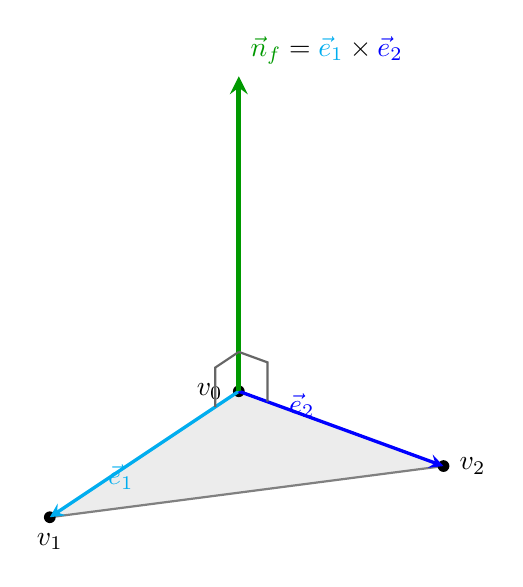
\begin{tikzpicture}[
    >=stealth,
    x={(-0.6cm, -0.4cm)}, y={(1cm, -0.1cm)}, z={(0cm, 1cm)},
    vec/.style={->, very thick},
    vertex/.style={circle, fill=black, inner sep=1.5pt}
]

% Coordinates in 3D
\coordinate (v0) at (0, 0, 0);
\coordinate (v1) at (4, 0, 0);  % Along X axis
\coordinate (v2) at (1.5, 3.5, 0);  % In XY plane

% Draw the triangle
\draw[fill=gray!15, draw=black!50, thick, join=round] (v0) -- (v1) -- (v2) -- cycle;

% Vertices
\node[vertex, label=left:{$v_0$}] at (v0) {};
\node[vertex, label=below:{$v_1$}] at (v1) {};
\node[vertex, label=right:{$v_2$}] at (v2) {};

% Vectors e1 and e2
\draw[vec, draw=cyan] (v0) -- (v1) node[midway, below left] {$\textcolor{cyan}{\vec{e}_1}$};
\draw[vec, draw=blue] (v0) -- (v2) node[midway, above left, xshift=-0.2cm] {$\textcolor{blue}{\vec{e}_2}$};

% Face normal
\coordinate (nf) at (0, 0, 4);
\draw[vec, draw=green!60!black, line width=1.8pt] (v0) -- (nf) node[above right] {$\textcolor{green!60!black}{\vec{n}_f} = \textcolor{cyan}{\vec{e}_1} \times \textcolor{blue}{\vec{e}_2}$};

% Right angle symbols in native 3D coordinates
% Between e1 (along X axis) and nf (along Z axis)
\draw[black!60, thick] (0.5, 0, 0) -- (0.5, 0, 0.5) -- (0, 0, 0.5);

% Between e2 (1.5, 3.5, 0) and nf (0, 0, 4)
% We move a bit along e2: let's use t = 0.14 -> (0.21, 0.49, 0)
\coordinate (e2_dir) at (0.21, 0.49, 0);
\coordinate (e2_dir_up) at (0.21, 0.49, 0.5);
\coordinate (z_dir) at (0, 0, 0.5);
\draw[black!60, thick] (e2_dir) -- (e2_dir_up) -- (z_dir);

\end{tikzpicture}
\caption{Visualization of the cross product calculation.}
\label{fig:face_normal}
\end{figure}

For a triangle with vertices $v_0$, $v_1$, $v_2$, the two edge vectors are:

\begin{equation}
    \textcolor{cyan}{\vec{e}_1} = v_1 - v_0, \qquad \textcolor{blue}{\vec{e}_2} = v_2 - v_0
\end{equation}

The area-weighted face normal is the cross product of these edges, resulting in a perpendicular vector:

\begin{equation}
    \textcolor{green!60!black}{\vec{n}_f} = \textcolor{cyan}{\vec{e}_1} \times \textcolor{blue}{\vec{e}_2}
\end{equation}

\begin{figure}[H]
\centering
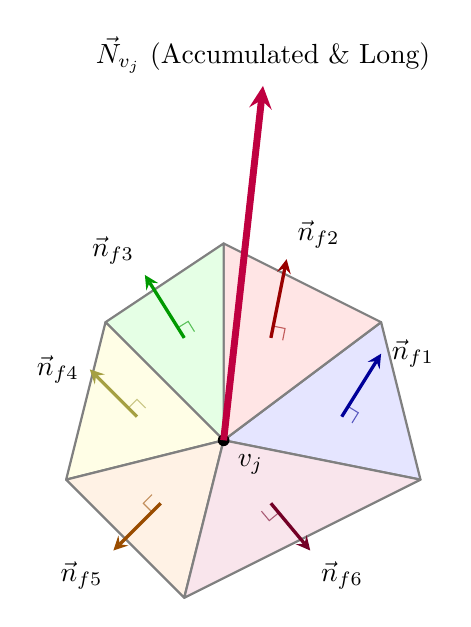
\begin{tikzpicture}[
    >=stealth,
    vec/.style={->, very thick},
    vertex/.style={circle, fill=black, inner sep=1.5pt}
]

% Central vertex
\coordinate (v) at (0, 0);

% Neighboring vertices (forming a fan around v)
\coordinate (n1) at (2.5, -0.5);
\coordinate (n2) at (2.0, 1.5);
\coordinate (n3) at (0.0, 2.5);
\coordinate (n4) at (-1.5, 1.5);
\coordinate (n5) at (-2.0, -0.5);
\coordinate (n6) at (-0.5, -2.0);

% Draw the faces
\draw[fill=blue!10, draw=black!50, thick, join=round] (v) -- (n1) -- (n2) -- cycle;
\draw[fill=red!10, draw=black!50, thick, join=round] (v) -- (n2) -- (n3) -- cycle;
\draw[fill=green!10, draw=black!50, thick, join=round] (v) -- (n3) -- (n4) -- cycle;
\draw[fill=yellow!10, draw=black!50, thick, join=round] (v) -- (n4) -- (n5) -- cycle;
\draw[fill=orange!10, draw=black!50, thick, join=round] (v) -- (n5) -- (n6) -- cycle;
\draw[fill=purple!10, draw=black!50, thick, join=round] (v) -- (n6) -- (n1) -- cycle;

% Central vertex node
\node[vertex, label=below right:{$v_j$}] at (v) {};

% f1: blue triangle (v, n1, n2), center approx (1.5, 0.3)
\draw[vec, draw=blue!60!black] (1.5, 0.3) -- (2.0, 1.1) node[right] {$\vec{n}_{f1}$};
\draw[thin, blue!60!black, opacity=0.6] (1.5, 0.3) ++(0.13, -0.08) -- ++(0.08, 0.13) -- ++(-0.13, 0.08);

% f2: red triangle (v, n2, n3), center approx (0.6, 1.3)
\draw[vec, draw=red!60!black] (0.6, 1.3) -- (0.8, 2.3) node[above right] {$\vec{n}_{f2}$};
\draw[thin, red!60!black, opacity=0.6] (0.6, 1.3) ++(0.15, -0.03) -- ++(0.03, 0.15) -- ++(-0.15, 0.03);

% f3: green triangle (v, n3, n4), center approx (-0.5, 1.3)
\draw[vec, draw=green!60!black] (-0.5, 1.3) -- (-1.0, 2.1) node[above left] {$\vec{n}_{f3}$};
\draw[thin, green!60!black, opacity=0.6] (-0.5, 1.3) ++(0.13, 0.08) -- ++(-0.08, 0.13) -- ++(-0.13, -0.08);

% f4: yellow triangle (v, n4, n5), center approx (-1.1, 0.3)
\draw[vec, draw=yellow!60!black] (-1.1, 0.3) -- (-1.7, 0.9) node[left] {$\vec{n}_{f4}$};
\draw[thin, yellow!60!black, opacity=0.6] (-1.1, 0.3) ++(0.11, 0.11) -- ++(-0.11, 0.11) -- ++(-0.11, -0.11);

% f5: orange triangle (v, n5, n6), center approx (-0.8, -0.8)
\draw[vec, draw=orange!60!black] (-0.8, -0.8) -- (-1.4, -1.4) node[below left] {$\vec{n}_{f5}$};
\draw[thin, orange!60!black, opacity=0.6] (-0.8, -0.8) ++(-0.11, 0.11) -- ++(-0.11, -0.11) -- ++(0.11, -0.11);

% f6: purple triangle (v, n6, n1), center approx (0.6, -0.8)
\draw[vec, draw=purple!60!black] (0.6, -0.8) -- (1.1, -1.4) node[below right] {$\vec{n}_{f6}$};
\draw[thin, purple!60!black, opacity=0.6] (0.6, -0.8) ++(-0.12, -0.10) -- ++(0.10, -0.12) -- ++(0.12, 0.10);

% Accumulated long vertex normal
\draw[vec, draw=purple, line width=2.5pt] (v) -- (0.5, 4.5) node[above] {$\vec{N}_{v_j}$ (Accumulated \& Long)};

\end{tikzpicture}
\caption{Visualization of Formula 3.4.}
\label{fig:accumulate_normal}
\end{figure}

The magnitude $|\vec{n}_f|$ equals twice the area of the triangle, so larger faces naturally contribute more weight. Each face normal is accumulated into its three vertices using atomic addition:

\begin{equation}
    \vec{N}_{v_j} = \sum_{f \in \mathcal{F}(v_j)} \vec{n}_f, \qquad j = 0, 1, 2
\end{equation}

where $\mathcal{F}(v_j)$ is the set of all faces adjacent to vertex $v_j$.

\begin{figure}[H]
\centering
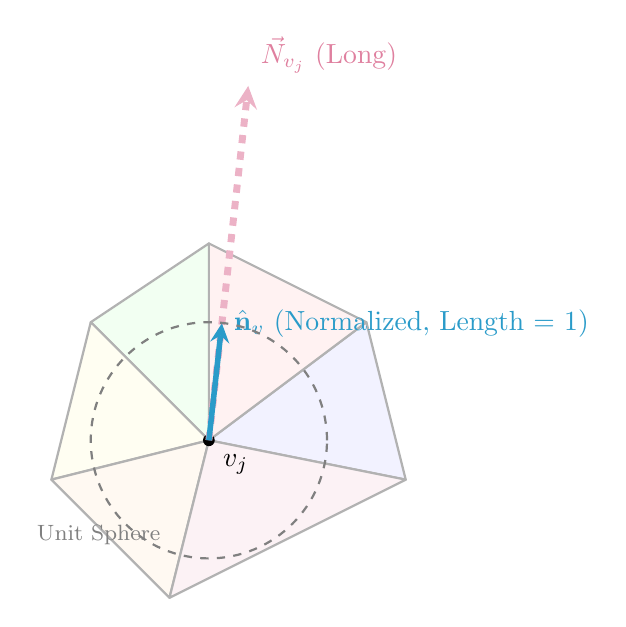
\begin{tikzpicture}[
    >=stealth,
    vec/.style={->, very thick},
    vertex/.style={circle, fill=black, inner sep=1.5pt}
]

% Central vertex
\coordinate (v) at (0, 0);

% Neighboring vertices (forming a fan around v)
\coordinate (n1) at (2.5, -0.5);
\coordinate (n2) at (2.0, 1.5);
\coordinate (n3) at (0.0, 2.5);
\coordinate (n4) at (-1.5, 1.5);
\coordinate (n5) at (-2.0, -0.5);
\coordinate (n6) at (-0.5, -2.0);

% Draw the faces (faded to emphasize the normal)
\draw[fill=blue!5, draw=black!30, thick, join=round] (v) -- (n1) -- (n2) -- cycle;
\draw[fill=red!5, draw=black!30, thick, join=round] (v) -- (n2) -- (n3) -- cycle;
\draw[fill=green!5, draw=black!30, thick, join=round] (v) -- (n3) -- (n4) -- cycle;
\draw[fill=yellow!5, draw=black!30, thick, join=round] (v) -- (n4) -- (n5) -- cycle;
\draw[fill=orange!5, draw=black!30, thick, join=round] (v) -- (n5) -- (n6) -- cycle;
\draw[fill=purple!5, draw=black!30, thick, join=round] (v) -- (n6) -- (n1) -- cycle;

% Central vertex node
\node[vertex, label=below right:{$v_j$}] at (v) {};

% Long accumulated normal
\draw[vec, draw=purple!30, line width=2.5pt, dashed] (v) -- (0.5, 4.5) node[above right, text=purple!50] {$\vec{N}_{v_j}$ (Long)};

% Short normalized normal (length = 1.5 for visual scale)
\draw[vec, draw=cyan!80!black, line width=2pt] (v) -- (0.165, 1.485) node[right, text=cyan!80!black] {$\hat{\mathbf{n}}_v$ (Normalized, Length = 1)};

% A circle of radius 1.5 to represent unit length
\draw[dashed, draw=gray, thick] (v) circle (1.5);
\node[text=gray, font=\footnotesize] at (-1.4, -1.2) {Unit Sphere};

\end{tikzpicture}
\caption{Visualization of Formula 3.5.}
\label{fig:normalize_normal}
\end{figure}

The final vertex normal is obtained by normalization:

\begin{equation}
    \hat{\mathbf{n}}_v = \frac{\vec{N}_v}{|\vec{N}_v|}, \qquad \text{or} \qquad (0, 0, 1) \quad \text{if } |\vec{N}_v| = 0
\end{equation}

Two CUDA kernels in \texttt{Core/ModelHelper.cu} handle this: \texttt{GPUNormalCaculation} uses \texttt{blockSize=256} and \texttt{atomicAdd} to accumulate face normals into vertex normals, and \texttt{GPUNormalizeVertexNormal} normalizes them to unit length. This runs on a dedicated CUDA stream in parallel with BVH construction.

\subsection{Build BVH}

If the SBT is the "address book" that tells the GPU what code to run, how does the ray actually find the triangle it hits in a scene with millions of them? Do we test the ray against every single triangle? Absolutely not! That would take forever. Instead, we use a clever sorting system called a Bounding Volume Hierarchy (BVH).


Think of the BVH like a massive game of "Guess Who?". Instead of asking "did I hit triangle 1? Did I hit triangle 2?", the BVH puts the whole 3D model inside a giant invisible box. It asks, "Did the ray hit the giant box?" If no, the ray missed completely! If yes, the BVH splits the box into two smaller boxes and asks again. It keeps splitting into smaller and smaller boxes until it finds the exact triangle the ray hit. This "divide and conquer" trick makes finding hits incredibly fast.



\begin{figure}[H]
    \centering
    
\includegraphics[width=0.8\textwidth]{"images/Chapter3/BVH constrution/Capture.PNG"}
    \caption{Visual representation of the Bounding Volume Hierarchy (BVH) structure.}
    \label{fig:bvh_structure}
\end{figure}

Figure \ref{fig:bvh_structure} illustrates this BVH structure. When we tell OptiX to build this BVH box system, we have to flip a special switch called "disable face culling." Why? Because normally, GPUs only let rays hit the outside of a 3D model. But for our thickness calculation, we are shooting rays *inside* the model! Flipping this switch lets our rays safely hit the back-walls on the inside.

The BVH is built by \texttt{OptixRunner::BuildBVH()} in \texttt{OptixRunner.cuh} using \texttt{optixAccelBuild}. Key flags: \texttt{OPTIX\_BUILD\_FLAG\_PREFER\_FAST\_TRACE} optimizes for trace speed, and \texttt{OPTIX\_GEOMETRY\_FLAG\_DISABLE\_TRIANGLE\_FACE\_CULLING} enables both-sided triangle hits for interior rays. This runs on a dedicated CUDA stream (\texttt{streamBVH}) in parallel with vertex normal computation.

\section{OptiX Ray Tracing Engine}

With our 3D model fully loaded into GPU memory and its surface normals pre-calculated, the foundation is set. The next step in our pipeline is the core physics simulation: shooting millions of rays to measure distances. To achieve this in real-time, we leverage the NVIDIA OptiX ray tracing engine, which requires a specific architectural setup to unleash its hardware-accelerated performance.

\subsection{Build Shader Binding Table}

With the mesh geometry and normals prepared, the OptiX ray tracing pipeline can be configured. But how does the GPU know what to do when a ray actually hits something? The answer lies in the Shader Binding Table (SBT).

In older graphics rendering (like traditional video games), things are drawn one by one in a predictable order. But with ray tracing, a ray bounces around unpredictably! A ray might hit a glass window, a brick wall, or simply miss everything and hit the sky. How can the GPU possibly know what code to run for each unique material when billions of rays are flying everywhere? However chaotic it seems, the GPU solves this using a massive, ultra-fast dictionary called the Shader Binding Table.

Think of the SBT as a giant address book on the GPU. Every entry in this address book has two parts. First, it contains the "Shader ID," which is basically a phone number telling the GPU exactly which piece of code to run (like "run the glass reflection code"). Second, it contains "Arguments," which are extra notes attached to that entry (like "this glass is tinted green"). This clever design means you don't need to write new code for every single object in your scene; you just change the notes in the address book!

But what about our SDF computation? Do we need a massively complex address book? Not at all! Because our entire 3D mesh is made of the exact same material, our address book only needs a single entry for each main task: one for shooting the ray, one for when it hits a triangle, and one for when it misses completely. We don't even need to store extra notes in the address book, because the only thing we care about is the distance the ray traveled, which is automatically carried back by the ray hit program.

\begin{figure}[H]
\centering
\resizebox{\textwidth}{!}{%
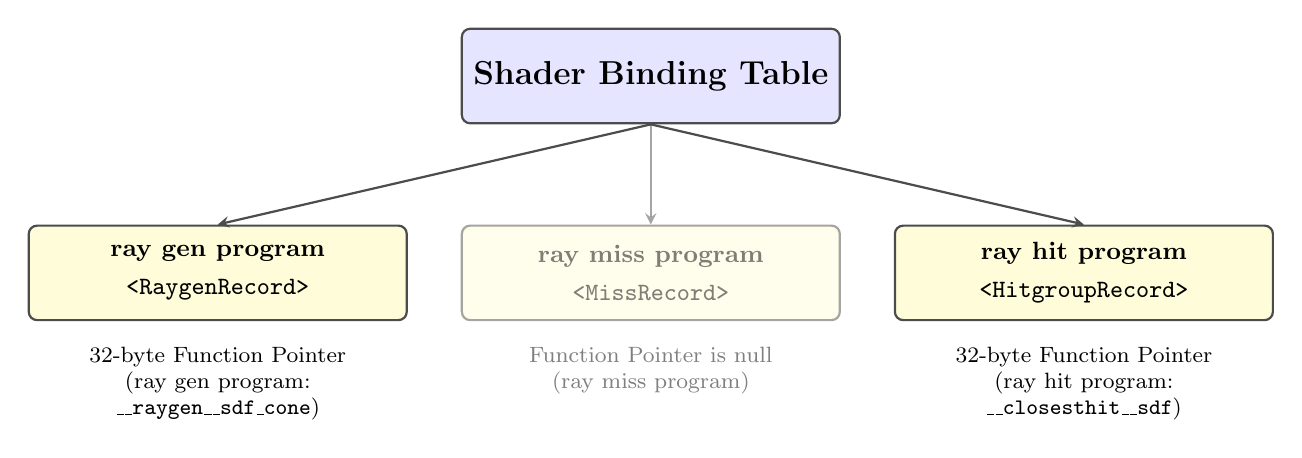
\begin{tikzpicture}[
    >=stealth,
    box/.style={
        rectangle, 
        rounded corners=3pt,
        draw=black!70, 
        thick, 
        minimum width=4.8cm, 
        minimum height=1.2cm,
        align=center,
        font=\small
    },
    sbtbox/.style={box, fill=blue!10},
    recbox/.style={box, fill=yellow!15},
    arrow/.style={->, thick, draw=black!70}
]

\node[sbtbox, font=\bfseries\large] (sbt) at (0, 0) {Shader Binding Table};

\node[recbox] (rg) at (-5.5, -2.5) {\textbf{ray gen program}\\[1mm]\texttt{<RaygenRecord>}};
\node[recbox, opacity=0.5] (ms) at (0, -2.5) {\textbf{ray miss program}\\[1mm]\texttt{<MissRecord>}};
\node[recbox] (hg) at (5.5, -2.5) {\textbf{ray hit program}\\[1mm]\texttt{<HitgroupRecord>}};

\draw[arrow] (sbt.south) -- (rg.north);
\draw[arrow, opacity=0.5] (sbt.south) -- (ms.north);
\draw[arrow] (sbt.south) -- (hg.north);

% Add details inside or below
\node[below=0.2cm of rg, font=\footnotesize, align=center] {32-byte Function Pointer\\(ray gen program:\\\texttt{\_\_raygen\_\_sdf\_cone})};
\node[below=0.2cm of ms, font=\footnotesize, align=center, opacity=0.5] {Function Pointer is null\\(ray miss program)};
\node[below=0.2cm of hg, font=\footnotesize, align=center] {32-byte Function Pointer\\(ray hit program:\\\texttt{\_\_closesthit\_\_sdf})};

\end{tikzpicture}%
}
\caption{Diagram of our Shader Binding Table implementation.}
\label{fig:sbt_architecture}
\end{figure}

Figure \ref{fig:sbt_architecture} demonstrates how it acts as an execution directory, mapping three distinct ray tracing events to their corresponding code on the GPU: generating the initial cone rays, recording distances when rays successfully hit the mesh, and correctly ignoring rays that miss the mesh entirely.

The SBT is constructed by \texttt{OptixRunner::BuildSBT()} in \texttt{OptixRunner.cuh}. Three records (\texttt{RaygenRecord}, \texttt{MissRecord}, \texttt{HitgroupRecord}) are packed with \texttt{optixSbtRecordPackHeader} and uploaded to device memory. Each record uses \texttt{OPTIX\_SBT\_RECORD\_ALIGNMENT} for proper GPU memory alignment.


\subsection{OptiX Pipeline Setup}

With the SBT configured, the OptiX pipeline itself must be initialized. The OptiX ray tracing pipeline is initialized once and reused for each model. It consists of a module creation step, program group definitions, and pipeline linking.

Now that the "address book" (SBT) and the "boxes" (BVH) are ready, we give OptiX three specific mini-programs to run. However, the OptiX engine cannot run raw C++ code directly. These mini-programs are written in OptiX CUDA C++ (\texttt{.cu} files) and must use the OptiX shader compiler to first be compiled into Parallel Thread Execution (PTX) format---an intermediate, assembly-like language designed specifically for NVIDIA GPUs. 

\begin{figure}[H]
\centering
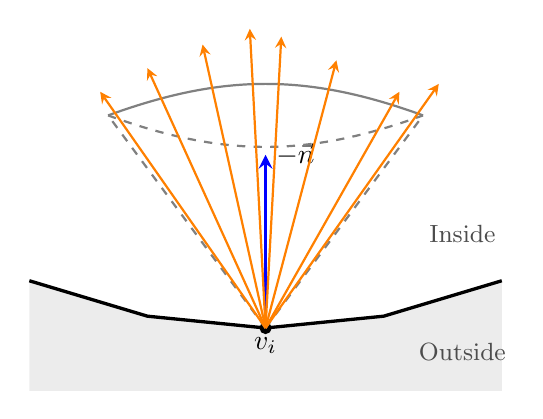
\begin{tikzpicture}[
    >=stealth,
    surface/.style={draw=black, very thick},
    ray/.style={->, draw=orange, thick}
]

% Gray out the outside of the model
\fill[gray!15] (-3, 0.4) -- (-1.5, -0.05) -- (0, -0.2) -- (1.5, -0.05) -- (3, 0.4) -- (3, -1.0) -- (-3, -1.0) -- cycle;

% Draw a polygonal surface representing the mesh triangles
\draw[surface] (-3, 0.4) -- (-1.5, -0.05) -- (0, -0.2) -- (1.5, -0.05) -- (3, 0.4);

% Labels for Inside and Outside
\node[font=\small, text=black!70] at (2.5, 1.0) {Inside};
\node[font=\small, text=black!70] at (2.5, -0.5) {Outside};

% Central vertex
\filldraw[black] (0, -0.2) circle (2pt) node[below] {$v_i$};

% Normal vector (pointing inward for our SDF)
\draw[->, draw=blue, very thick] (0, -0.2) -- (0, 2) node[right] {$-\vec{n}$};

% Cone boundary
\draw[draw=gray, dashed, thick] (0, -0.2) -- (-2, 2.5);
\draw[draw=gray, dashed, thick] (0, -0.2) -- (2, 2.5);
\draw[draw=gray, thick] (-2, 2.5) to[out=20, in=160] (2, 2.5);
\draw[draw=gray, thick, dashed] (-2, 2.5) to[out=-20, in=-160] (2, 2.5);

% Random rays inside the cone, passing further through the cone's base
\draw[ray] (0, -0.2) -- (-1.5, 3.1);
\draw[ray] (0, -0.2) -- (-0.8, 3.4);
\draw[ray] (0, -0.2) -- (0.2, 3.5);
\draw[ray] (0, -0.2) -- (0.9, 3.2);
\draw[ray] (0, -0.2) -- (1.7, 2.8);
\draw[ray] (0, -0.2) -- (-2.1, 2.8);
\draw[ray] (0, -0.2) -- (2.2, 2.9);
\draw[ray] (0, -0.2) -- (-0.2, 3.6);



\end{tikzpicture}
\caption{The Ray Generator program scatters 64 rays in a conical distribution around the vertex normal, sending them inward to measure the distance to the opposite side of the mesh.}
\label{fig:raygen_diagram}
\end{figure}

The Ray Generator program creates the rays. Instead of shooting just one ray straight down, it randomly scatters 64 rays in a cone shape (like a shotgun blast) pointing inside the model. When a ray hits something, this program records how far it traveled.


Once a ray is generated and sent into the BVH, OptiX traverses the acceleration structure to find the nearest intersection. When the ray strikes the closest triangle, the \textbf{Closest-Hit Program} is triggered. Its entire purpose is astonishingly simple: it immediately queries the ray's maximum traveled distance (using the hardware-accelerated \texttt{optixGetRayTmax()}) and writes this raw float value directly into the ray's 32-bit payload. This single piece of data is then automatically carried back to the Ray Generator, giving us exactly the thickness measurement we need.

Normally, when a ray travels through a scene, an Any-Hit program is triggered every single time the ray crosses *any* potential surface along its path, before it finds the final solid wall. This is extremely useful for things like transparent glass or leaves with see-through holes, because the Any-Hit program can check if the ray should pass straight through the transparent parts. 

However, OptiX is extremely fast because we use a special trick: we completely disable these Any-Hit programs. Why? Because our 3D models are completely solid and opaque! Evaluating transparency at every single intersection is a huge waste of time. By disabling it, we let the specialized hardware RT Cores run at maximum speed and blast straight to the closest wall without stopping to ask questions. Finally, we tell OptiX to only let rays bounce once. We don't care about reflections; we just want to know where the inside wall is!

The pipeline is created by \texttt{OptixRunner::CreatePipeline()} in \texttt{OptixRunner.cuh}. The PTX code is JIT-compiled via \texttt{optixModuleCreate}, then three program groups are created with entry functions \texttt{\_\_raygen\_\_sdf\_cone} and \texttt{\_\_closesthit\_\_sdf}. Key parameters: \texttt{maxTraceDepth=1}, \texttt{numPayloadValues=1}, \texttt{raysPerPoint=64}, cone angle $= 150^\circ$, Hammersley quasi-random sampling, and \texttt{OPTIX\_RAY\_FLAG\_DISABLE\_ANYHIT} for maximum RT Core throughput.

\subsection{Calculate Weighted SDF}

Once all the rays are finished flying around, we have a massive pile of hit distances. But remember, rays shooting straight down the middle are more trustworthy than rays shooting out at wide angles. So, we pass all these distances into a final math formula to calculate a "weighted average" for every point on the model.

\begin{equation}
    \mathrm{SDF}(p) = \frac{\sum_{i=1}^{R_p} d_i \cdot w_i}{\sum_{i=1}^{R_p} w_i}
    \label{eq:sdf_formula}
\end{equation}

If a ray missed and returned a "-1", we simply throw it in the trash. If every single ray for a point missed, we just assign it a thickness of zero. 

The \texttt{GPUComputeRawSDF} kernel in \texttt{SDFKernels.cuh} computes the weighted average for each vertex using \texttt{blockSize=256}. Each vertex's raw SDF is calculated as shown in Equation~\ref{eq:sdf_formula}, where the weight $w_i$ is the inverse of the angle between the ray and the cone axis.

\section{GPU Post-Processing}

After the OptiX pipeline completes its ray tracing, we are left with a raw collection of distance values. However, directly rendering these raw values often results in a visual representation that is noisy and difficult to interpret. To transform these raw distances into a clean, smooth, and visually intuitive heat map, we rely on a dedicated GPU post-processing stage. Because the first two steps---normalizing the SDF values and building the adjacency graph (CSR format)---are entirely independent, we execute them simultaneously using separate CUDA streams to maximize hardware utilization before the final smoothing step.

\begin{figure}[H]
    \centering
    \begin{tabular}{@{}c@{}}
        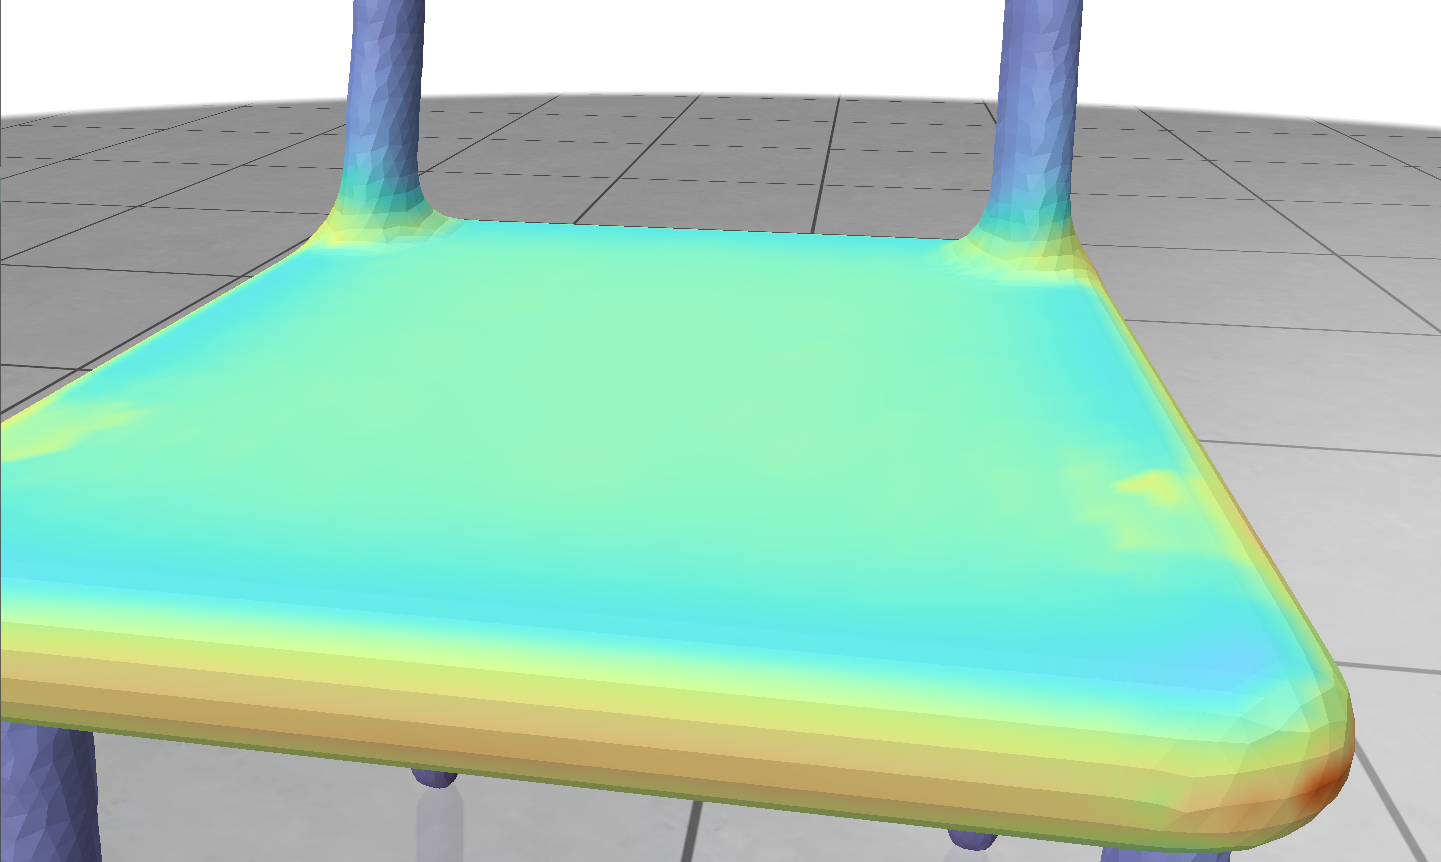
\includegraphics[width=0.6\textwidth]{images/Chapter3/postProcess/no_normalization.png} \\
        \textbf{(a) Raw SDF} \\[3ex]
        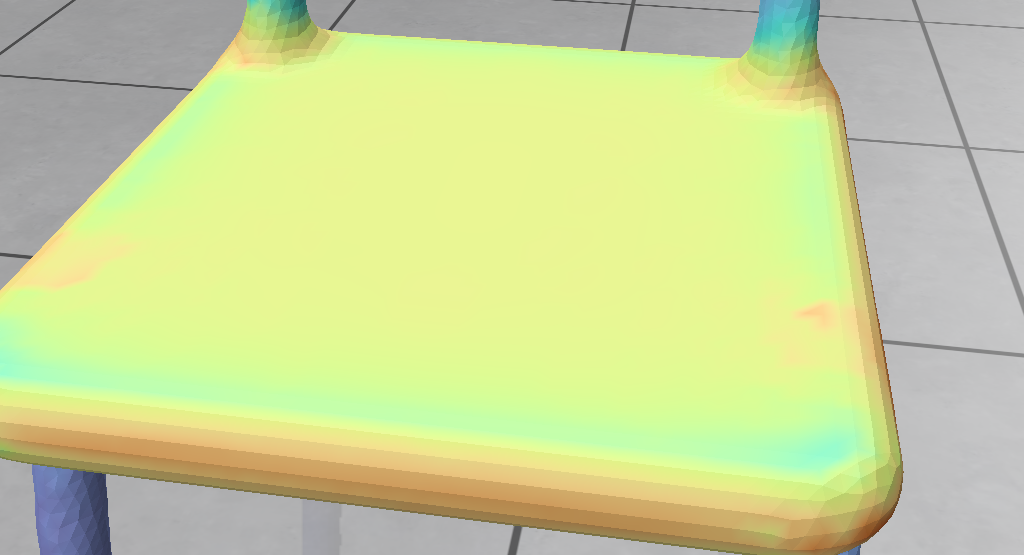
\includegraphics[width=0.6\textwidth]{images/Chapter3/postProcess/normalization.png} \\
        \textbf{(b) Normalized} \\[3ex]
        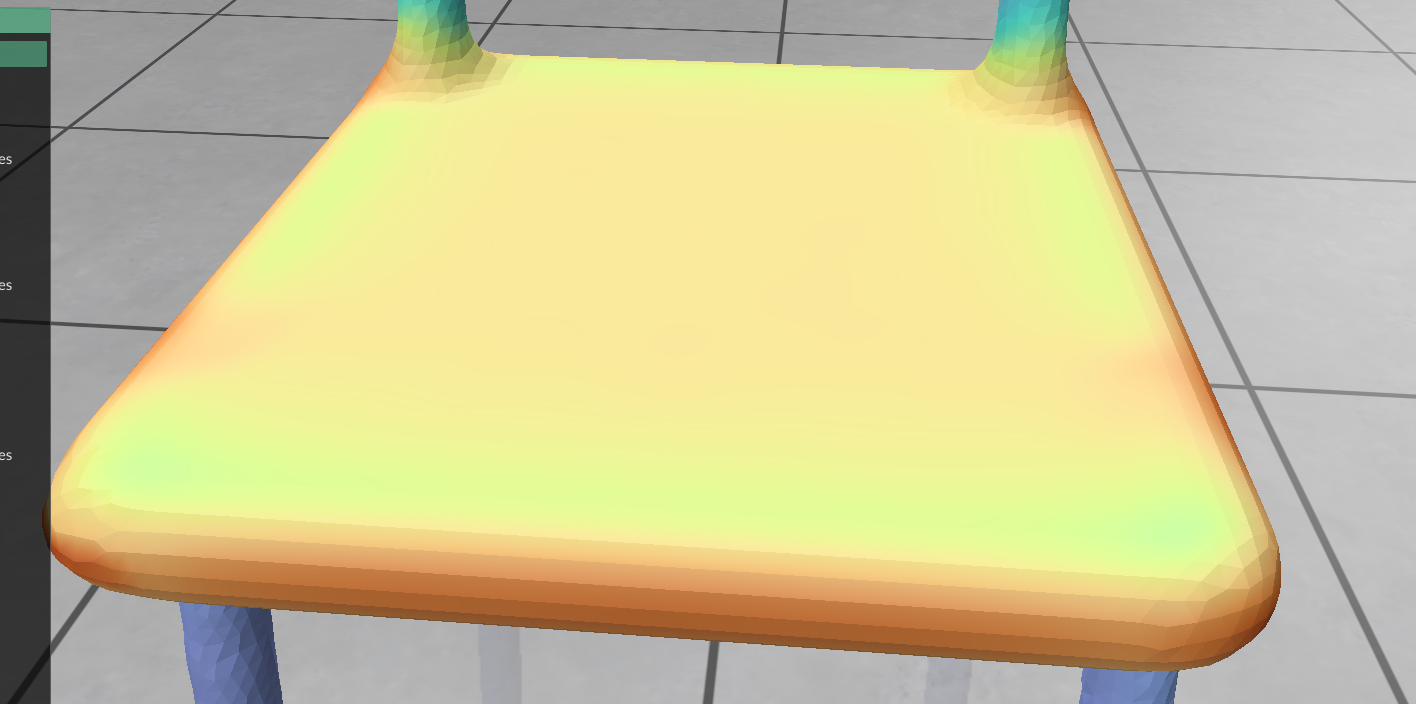
\includegraphics[width=0.6\textwidth]{images/Chapter3/postProcess/smoothed.png} \\
        \textbf{(c) Smoothed}
    \end{tabular}
    \caption{The step-by-step SDF transformation pipeline.}
    \caption*{Starting from the raw SDF, we apply normalization to map the values to a usable range, and finally execute an anisotropic smoothing pass to eliminate noise while preserving sharp features.}
    \label{fig:postprocess_pipeline}
\end{figure}

\subsection{Normalize SDF}

However, the raw thickness numbers we just calculated might range from 0.001 to 500.0, which makes them hard to colorize or display nicely. To fix this, we "normalize" the numbers. This is a fancy way of saying we squash all the numbers so that the thinnest point is exactly 0.0 and the thickest point is exactly 1.0. We also use a math trick called "logarithmic compression" which helps us preserve the tiny details in thin areas (like fingers) so they don't get drowned out by massive areas (like the torso).

\begin{equation}
    \hat{v} = \frac{\mathrm{SDF}(p) - \mathrm{SDF}_{\min}}{\mathrm{SDF}_{\max} - \mathrm{SDF}_{\min}}, \qquad
    v_{\mathrm{norm}} = \frac{\log(4.0 \cdot \hat{v} + 1)}{\log(4.0 + 1)}
\end{equation}

The normalization pipeline in \texttt{SDFKernels.cuh} runs three CUDA kernels sequentially: \texttt{GPUComputeBoundingBox} finds the axis-aligned bounding box, \texttt{GPUComputeSDFMinMax} finds the minimum and maximum SDF values, and \texttt{GPUApplySDFNormalization} applies logarithmic compression with $\alpha = 4.0$. This runs on \texttt{streamNorm} in parallel with adjacency graph construction.

\subsection{Build Adjacency Graph}

Even after normalization, our thickness values might look a bit noisy or splotchy. To fix this, we want to smooth them out by blending each point with its neighbors. But here's the trick: how does the GPU know who a point's neighbors are? 

We have to build a "friend list" for every point on the model. Formally, we represent the 3D mesh as a graph where vertices are nodes and the triangle edges connecting them are the graph's edges. A naive way to store this is a massive grid checking every point against every other point, called the adjacency matrix. For a graph with $|V|$ vertices, the adjacency matrix $A$ is a $|V| \times |V|$ square matrix where the element $A_{i,j}$ is $1$ if there is an edge connecting vertex $i$ to vertex $j$, and $0$ otherwise.

This requires $O(|V|^2)$ space complexity. This is absolutely catastrophic for large models because a typical vertex is only neighbors with a handful of other vertices (usually around 6), meaning the vast majority of the matrix is filled with zeros! Allocating memory for a full matrix would mean storing billions of zero values, wasting precious GPU VRAM and bandwidth. For example, here is a small adjacency matrix where the 0s (representing no connection, and therefore wasted space on the GPU) are colored red:

\begin{equation}
\label{eq:adj_matrix}
A = \begin{bmatrix}
1 & 1 & \textcolor{red}{0} & \textcolor{red}{0} \\
1 & 1 & 1 & \textcolor{red}{0} \\
\textcolor{red}{0} & 1 & 1 & 1 \\
\textcolor{red}{0} & \textcolor{red}{0} & 1 & 1
\end{bmatrix}
\end{equation}

Instead, we use a clever format called CSR (Compressed Sparse Row). It basically crushes the friend list down into a single, tightly packed line of data, skipping all the red zeros. This drops the memory complexity from $O(|V|^2)$ down to $O(|V|)$, which keeps the memory usage tiny and makes the GPU extremely happy because it doesn't have to jump around to find data.

To achieve this compression, we must first sort the edges. Why? Because the GPU generates edges randomly as it reads triangles, but the CSR format requires all of vertex $i$'s friends to be grouped together sequentially in memory. Once sorted, the CSR format splits the matrix into three separate 1D arrays. The \texttt{values} array stores only the non-zero elements from left to right, top to bottom. In our adjacency matrix, these are all the $1$s indicating that an edge connection exists. The \texttt{col\_ind} (Column Indices) array stores the original column number for every entry in the \texttt{values} array, telling us exactly \textit{which} vertex is the neighbor. The \texttt{row\_ptr} (Row Pointers) array acts as a master index where the $i$-th entry tells the GPU the exact starting position of vertex $i$'s friend list inside the \texttt{col\_ind} array. By looking at the difference between \texttt{row\_ptr}[$i+1$] and \texttt{row\_ptr}[$i$], the GPU instantly knows exactly how many neighbors vertex $i$ has.

\begin{figure}[H]
\centering
\resizebox{\textwidth}{!}{%
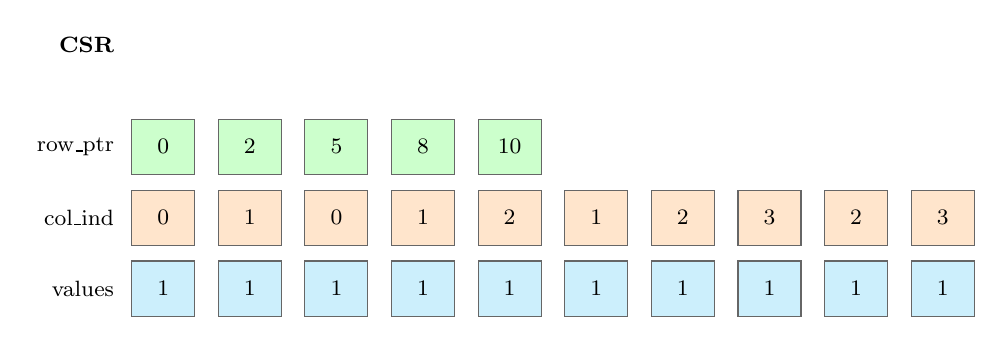
\begin{tikzpicture}[
    >=stealth,
    box/.style={rectangle, draw=black!60, fill=blue!8, minimum width=0.8cm, minimum height=0.7cm, font=\footnotesize, anchor=center},
    arr/.style={->, thick, gray}
]

% The sparse matrix visual has been removed; only the CSR arrays remain.

% CSR arrays
\node[font=\footnotesize\bfseries, anchor=east] at (4.5, 2.5) {CSR};

% row_ptr
\node[font=\footnotesize, anchor=east] at (4.5, 1.2) {row\_ptr};
\foreach \val [count=\i from 0] in {0,2,5,8,10} {
    \node[box, fill=green!20] at (5.0 + \i*1.1, 1.2) {\val};
}

% col_ind
\node[font=\footnotesize, anchor=east] at (4.5, 0.3) {col\_ind};
\foreach \val [count=\i from 0] in {0,1,0,1,2,1,2,3,2,3} {
    \node[box, fill=orange!20] at (5.0 + \i*1.1, 0.3) {\val};
}

% values
\node[font=\footnotesize, anchor=east] at (4.5, -0.6) {values};
\foreach \val [count=\i from 0] in {1,1,1,1,1,1,1,1,1,1} {
    \node[box, fill=cyan!20] at (5.0 + \i*1.1, -0.6) {\val};
}

% Mapping arrows removed per user request

\end{tikzpicture}%
}
\caption{CSR (Compressed Sparse Row) memory layout for the adjacency matrix in Equation \ref{eq:adj_matrix}.}
\label{fig:csr_layout}
\end{figure}

Figure \ref{fig:csr_layout} depicts how the 2D adjacency matrix is flattened into three dense 1D arrays. The \texttt{row\_ptr} array indicates the starting index of each vertex's neighbor list, the \texttt{col\_ind} array stores the actual neighbor vertex indices, and the \texttt{values} array holds the connection flags (which are all $1$ in our unweighted graph).

This is built entirely on the GPU using three steps in \texttt{SDFKernels.cuh}. First, the \texttt{GPUGenerateEdges} kernel generates 6 directed edges per triangle face (because a triangle has 3 undirected edges, and we need 2 directed edges---one in each direction---for every undirected edge to allow two-way neighbor lookups). Then, NVIDIA's CUB library sorts and deduplicates these edges via \texttt{cub::DeviceRadixSort} and \texttt{cub::DeviceSelect::Unique}. Finally, \texttt{GPUExtractCSR} converts the sorted unique edges into CSR arrays: \texttt{d\_nbrOffsets[V+1]} and \texttt{d\_nbrLists}. This runs on a dedicated \texttt{streamCSR} in parallel with normalization.

\subsection{Smooth SDF}

Now that we know everyone's neighbor, we can apply our smoothing filter. But we don't want a standard "blur" filter. A basic blur would smear the thickness values across sharp edges, turning crisp details into a muddy mess. Instead, we use an "Anisotropic Bilateral Filter". 

This sounds complicated, but it's actually very intuitive. It blends points together, but only if they are physically close to each other AND they have a similar thickness value. If two points are right next to each other but one is super thick and the other is super thin (like a sharp edge), the filter says "Stop! Don't blend these!" and leaves the sharp edge perfectly crisp. 

We use a fancy mathematical formula to calculate exactly how much to blend these points together:

\begin{equation}
    v_p^{\mathrm{out}} = \frac{\sum_{q \in \mathcal{N}(p)} \exp\!\left(-\frac{\|\mathbf{x}_p - \mathbf{x}_q\|^2}{2\sigma_s^2}\right) \exp\!\left(-\frac{(v_p - v_q)^2}{2\sigma_r^2}\right) v_q}{\sum_{q \in \mathcal{N}(p)} \exp\!\left(-\frac{\|\mathbf{x}_p - \mathbf{x}_q\|^2}{2\sigma_s^2}\right) \exp\!\left(-\frac{(v_p - v_q)^2}{2\sigma_r^2}\right)}
\end{equation}

Why the scary exponential ($\exp$) math? It acts like a smooth dimmer switch. Instead of a hard cut-off (like "blend 100\% if close, 0\% if far"), it smoothly fades the blending power the further away a friend gets. You might also notice the $2\sigma^2$ at the bottom of the fractions. This acts as our main control knob (derived from the variance of a Gaussian bell curve). A small $\sigma$ makes the dimmer switch drop to 0\% very quickly, while a large $\sigma$ creates a very long, smooth fade-out across many neighbors. By running this dimmer-switch filter over the whole mesh a few times, we get a gorgeous, noise-free thickness map that still preserves all the sharp, realistic details of the 3D model!

This is implemented in the \texttt{AnisotropicSmoothingKernel} CUDA kernel in \texttt{SDFKernels.cuh}. We run 3 smoothing iterations with \texttt{sigmaSpatial} set to 2\% of the model's bounding box diagonal, and \texttt{sigmaRange} set to 0.1. To avoid read-write conflicts, we use a double-buffered ping-pong approach (\texttt{d\_sdfBuf1} $\leftrightarrow$ \texttt{d\_sdfBuf2}), swapping input and output between each iteration.


% CHAPTER 4: EXPERIMENT RESULTS
\chapter{Experiment Results}

This chapter presents the experimental results of the proposed OptiX-based SDF computation pipeline. We describe the testing methodology, analyze the time complexity and real-time performance compared to the PyMeshLab GPU implementation, and evaluate the visual quality of the computed SDF values.

\section{Testing Method}

The experiments were conducted on a system equipped with an NVIDIA RTX GPU using CUDA and OptiX RT Cores. Two implementations were benchmarked: the proposed OptiX-based pipeline and the PyMeshLab GPU implementation (VCGlib/OpenGL). Both implementations used identical SDF parameters: 64 rays per vertex, a cone angle of 150 degrees, depth peeling iterations = 10 (higher values are needed for bigger models, but we fixed it for the sake of testing the framework easier), and no outlier removal. The OptiX pipeline included full post-processing (log normalization and 3 iterations of anisotropic bilateral smoothing), while PyMeshLab produced raw SDF values without post-processing. Timing was measured using \texttt{std::chrono::high\_resolution\_clock} for OptiX and \texttt{time.perf\_counter()} for PyMeshLab, with visualization disabled in both cases.

After the smoothed SDF values are computed, the results are visualized and compared against the reference implementation. The final SDF values are visualized as vertex-colored heat maps using Polyscope, a 3D geometry processing viewer. The \texttt{turbo} colormap maps normalized SDF values from blue (thin) to red (thick). Three models are displayed simultaneously for comparison. The OptiX SDF represents the smoothed result from the proposed pipeline. The PyMeshLab SDF is the reference result computed using VCGlib's OpenGL rasterization with identical parameters ($R = 64$, $\theta_{\mathrm{cone}} = 150^\circ$). The Difference model shows the absolute per-vertex difference $|v_{\mathrm{optix}} - v_{\mathrm{pymeshlab}}|$ for accuracy assessment.

\section{Time Complexity and Real-Time Speed Comparison}

The time complexity analysis reveals fundamental differences between the two approaches. Let $V$ = number of vertices, $F$ = number of faces, $R$ = rays per vertex, $N$ = number of camera directions, $P$ = depth peeling iterations (the bigger the model, the more peeling iterations it needs), $I$ = smoothing iterations, and $k$ = average neighbors per vertex.

The OptiX pipeline has total complexity $O(V \times R \times \log F + F \log F)$, dominated by BVH construction and ray tracing. Each vertex independently shoots $R$ rays through the hardware BVH, with each ray traversing the BVH in $O(\log F)$. The VCGlib/MeshLab GPU approach has total complexity $O(N \times (F \times P + V))$, dominated by depth peeling across all camera directions. Each of the $N$ directions requires a full mesh render pass with $P$ depth peeling layers.

Despite the $\log F$ factor in OptiX, it outperforms VCGlib because: (1) OptiX launches $V$ threads in parallel with RT Cores handling ray-BVH traversal in hardware, while VCGlib requires $N$ draw calls with fixed overhead; (2) OptiX uses zero-copy CUDA device pointers with no host-device transfer, while VCGlib requires \texttt{glReadPixels} readback; (3) OptiX's post-processing adds negligible cost compared to ray tracing, while VCGlib has no post-processing at all.

Table~\ref{tab:benchmark} shows the benchmark results across 12 models, comparing the execution time of the PyMeshLab GPU implementation against the proposed OptiX pipeline. OptiX is faster across all models, with speedups ranging from 3.1x to 171x. The table lists each model name, its vertex count, the execution time for both implementations in seconds, and the resulting speedup factor.

\begin{table}[ht]
\centering
\begin{tabular}{@{}lrrrr@{}}
\toprule
\textbf{Model} & \textbf{Vertices} & \textbf{PyMeshLab (s)} & \textbf{OptiX (s)} & \textbf{Speedup} \\
\midrule
360.obj & 2,200 & 0.3228 & 0.0019 & 171.0x \\
9.obj & 2,639 & 0.4359 & 0.0084 & 51.6x \\
400.obj & 3,703 & 0.4004 & 0.0121 & 33.2x \\
76.obj & 5,923 & 0.5027 & 0.0106 & 47.6x \\
181.obj & 7,242 & 0.3128 & 0.0039 & 80.6x \\
118.obj & 9,153 & 0.3141 & 0.0047 & 66.3x \\
368.obj & 11,202 & 0.3217 & 0.0163 & 19.7x \\
112.obj & 13,628 & 0.8288 & 0.0229 & 36.1x \\
369.obj & 13,606 & 0.3772 & 0.0517 & 7.3x \\
158.obj & 14,587 & 0.3450 & 0.0069 & 50.0x \\
371.obj & 14,599 & 0.3097 & 0.0583 & 5.3x \\
Leaf.obj & 24,866 & 0.3827 & 0.1219 & 3.1x \\
\bottomrule
\end{tabular}
\caption{Performance benchmark: PyMeshLab GPU vs.\ OptiX}
\label{tab:benchmark}
\end{table}

PyMeshLab GPU has a approximately 0.3s base overhead regardless of model size, due to OpenGL context initialization, texture upload, and iterating over 128 camera directions. OptiX scales better as its ray tracing time grows proportionally with vertex count, while PyMeshLab's overhead is dominated by fixed-cost OpenGL operations.

\section{Quality Comparison}

The visual quality of the computed SDF values was evaluated by comparing the OptiX results against the PyMeshLab GPU reference. Each comparison shows the SDF heat map from both implementations and their absolute difference per vertex. Hot colors (red/yellow) indicate larger SDF values (thicker regions), while cool colors (blue) indicate thinner regions.

Figure~\ref{fig:quality_112} through Figure~\ref{fig:quality_368} show the comparison results for representative models. The OptiX pipeline produces SDF values that closely match the PyMeshLab reference, with the difference maps showing minimal variation. The OptiX SDF is much smoother than the PyMeshLab result due to the anisotropic bilateral smoothing applied in the post-processing stage, which reduces noise while preserving features.

\begin{figure}[ht]
\centering
\begin{tabular}{@{}c@{}}
\cellcolor{red!15}\textbf{OptiX} \\
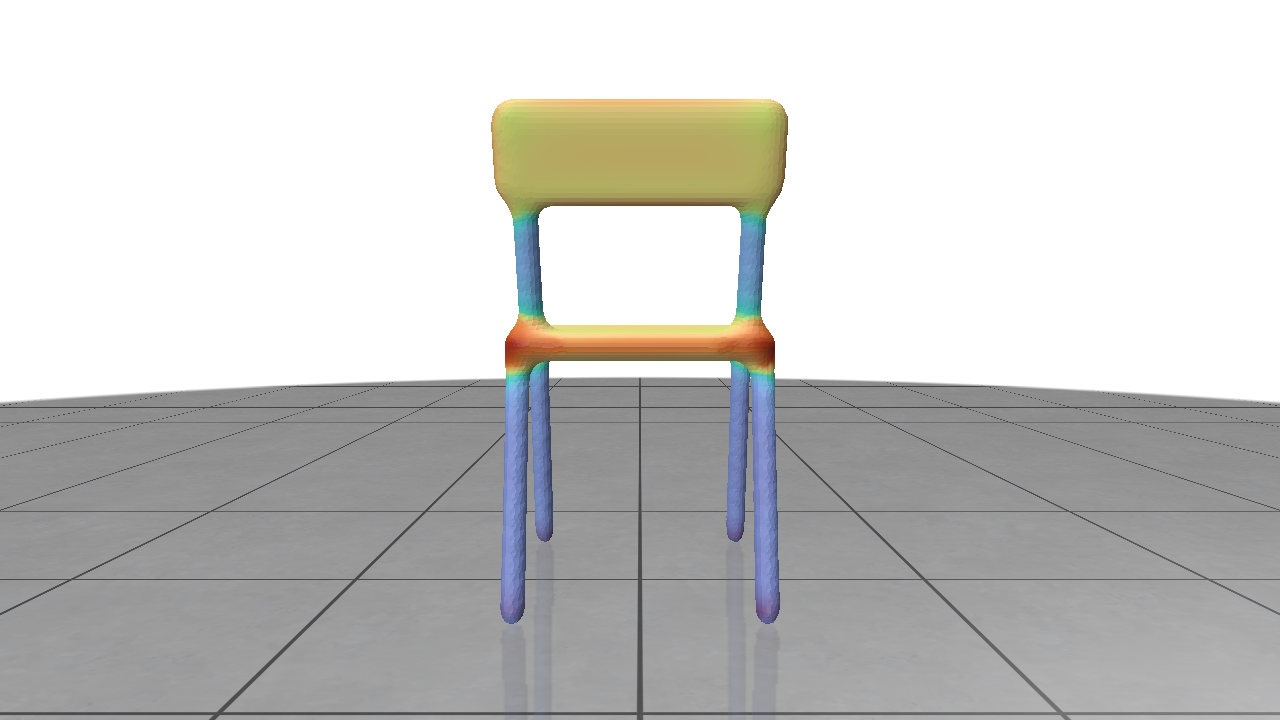
\includegraphics[width=0.65\textwidth]{../image/112_optix.png} \\
\cellcolor{green!15}\textbf{PyMeshLab} \\
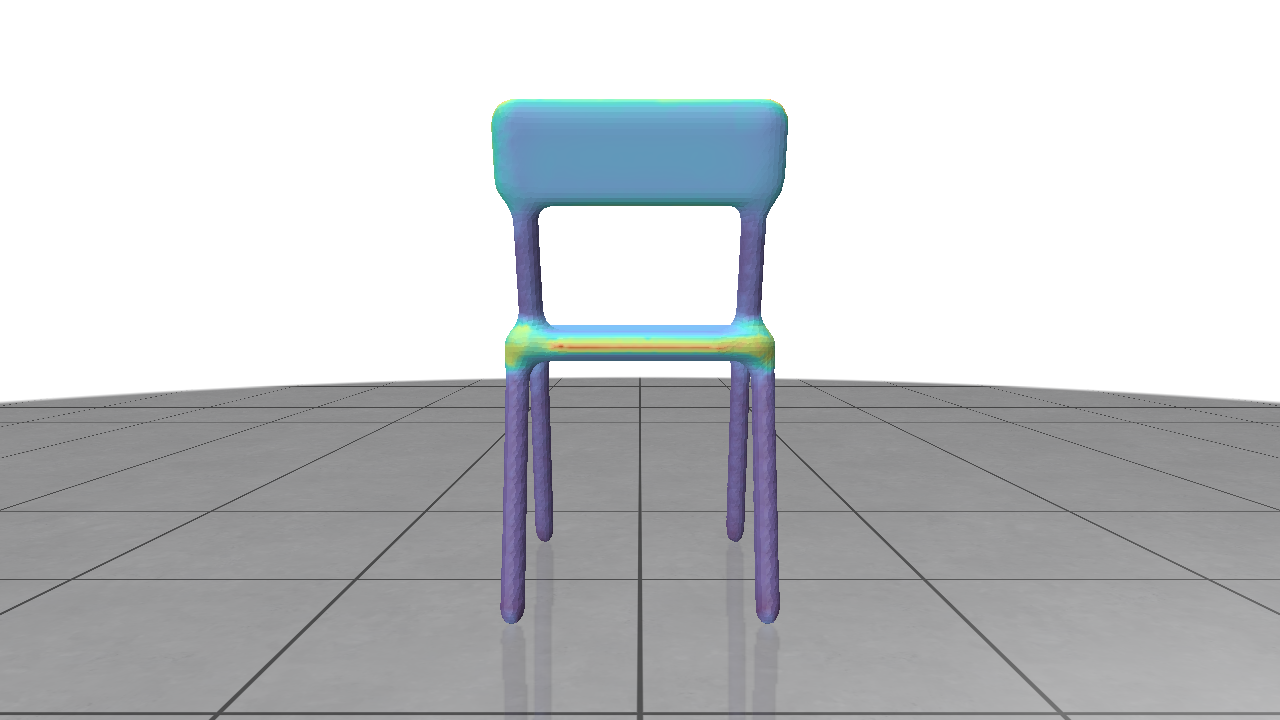
\includegraphics[width=0.65\textwidth]{../image/112_pymeshlab.png} \\
\cellcolor{blue!15}\textbf{Difference} \\
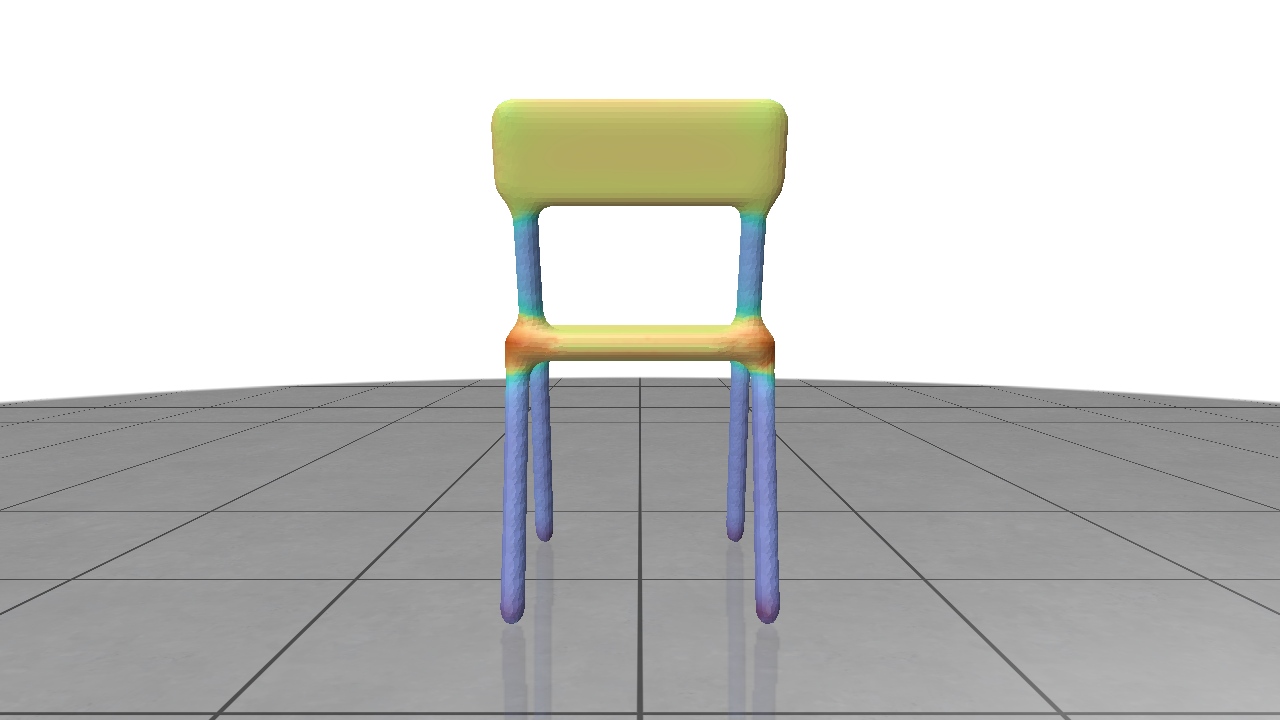
\includegraphics[width=0.65\textwidth]{../image/112_diff.png} \\
\end{tabular}
\caption{SDF quality comparison for model 112.obj (13,628 vertices)}
\label{fig:quality_112}
\end{figure}

Model 112 is one of the larger models in the dataset. The OptiX result shows a smooth, coherent heat map with well-defined thickness gradients across the surface. The PyMeshLab result exhibits slight noise in the thickness transitions. The difference map confirms that the discrepancy is minimal, with the largest deviations occurring at thin structural features where the bilateral smoothing in OptiX preserves edges more effectively.

\begin{figure}[ht]
\centering
\begin{tabular}{@{}c@{}}
\cellcolor{red!15}\textbf{OptiX} \\
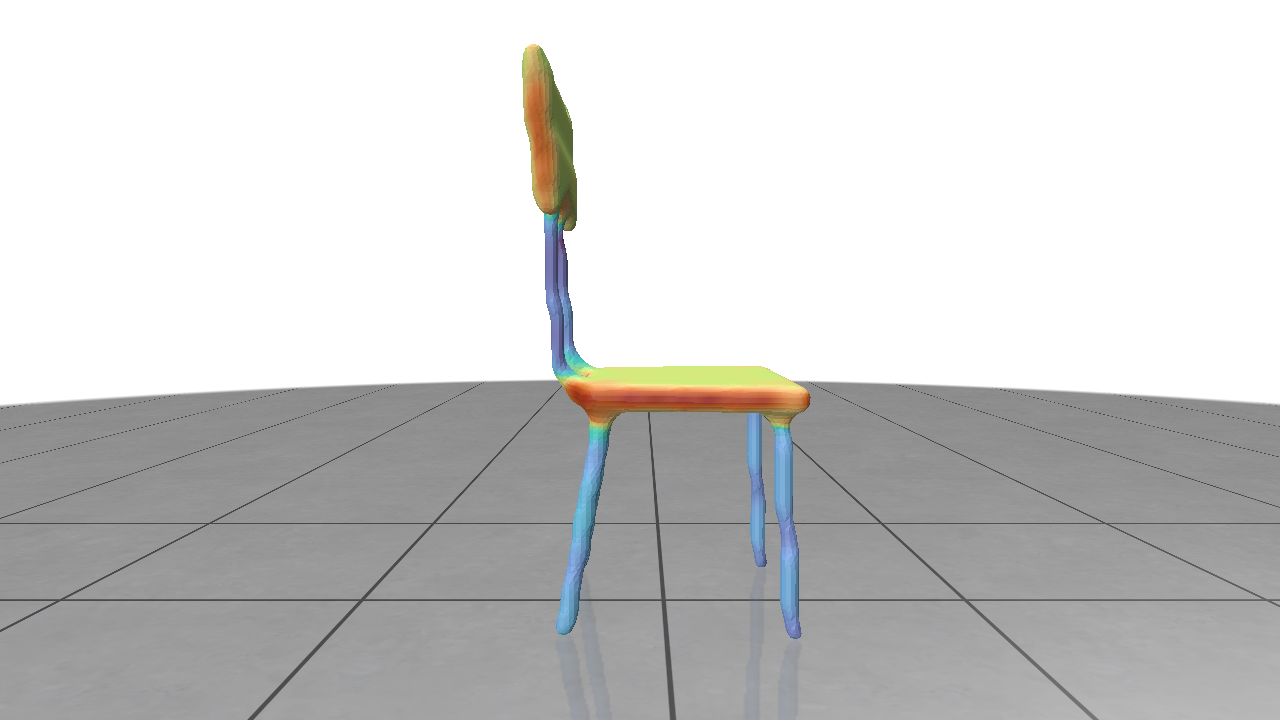
\includegraphics[width=0.65\textwidth]{../image/118_optix.png} \\
\cellcolor{green!15}\textbf{PyMeshLab} \\
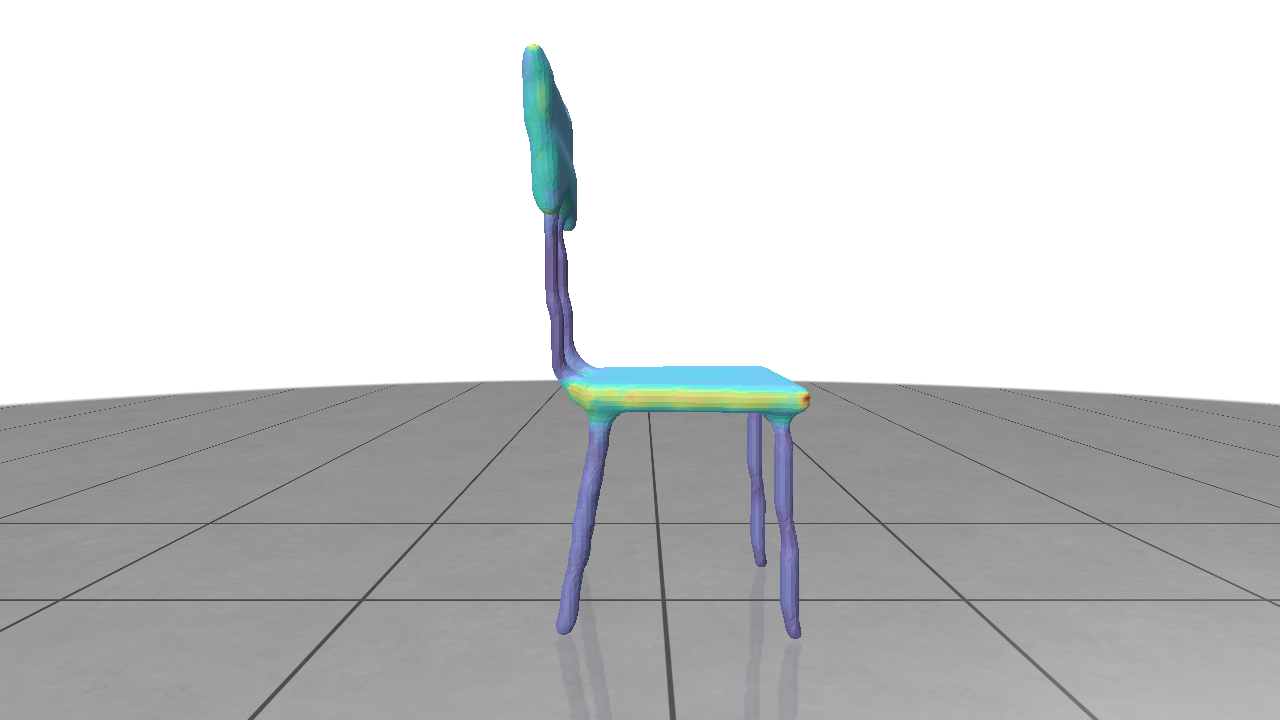
\includegraphics[width=0.65\textwidth]{../image/118_pymeshlab.png} \\
\cellcolor{blue!15}\textbf{Difference} \\
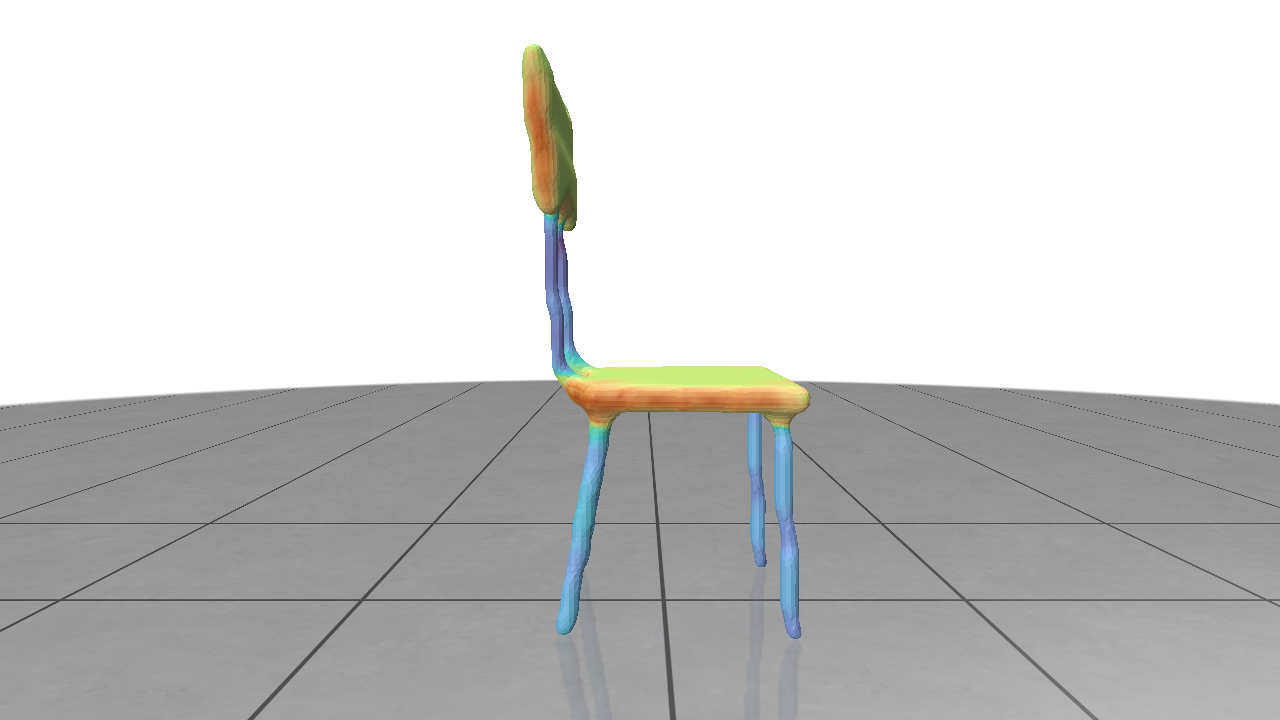
\includegraphics[width=0.65\textwidth]{../image/118_diff.png} \\
\end{tabular}
\caption{SDF quality comparison for model 118.obj (9,153 vertices)}
\label{fig:quality_118}
\end{figure}

Model 118 has a moderate vertex count and exhibits complex surface curvature. The OptiX heat map shows smooth thickness variation across curved regions, while the PyMeshLab result displays minor artifacts in areas of high curvature. The difference map indicates that both implementations agree on the overall thickness distribution, with discrepancies confined to local surface features.

\begin{figure}[ht]
\centering
\begin{tabular}{@{}c@{}}
\cellcolor{red!15}\textbf{OptiX} \\
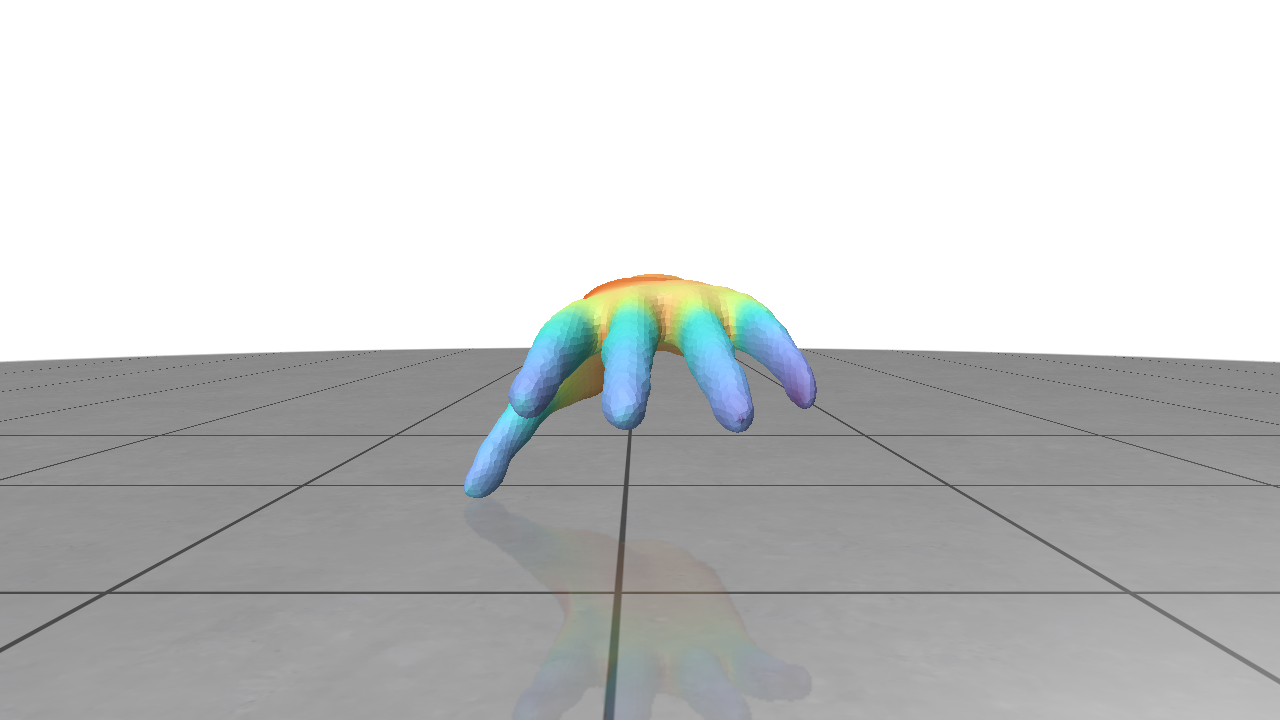
\includegraphics[width=0.65\textwidth]{../image/181_optix.png} \\
\cellcolor{green!15}\textbf{PyMeshLab} \\
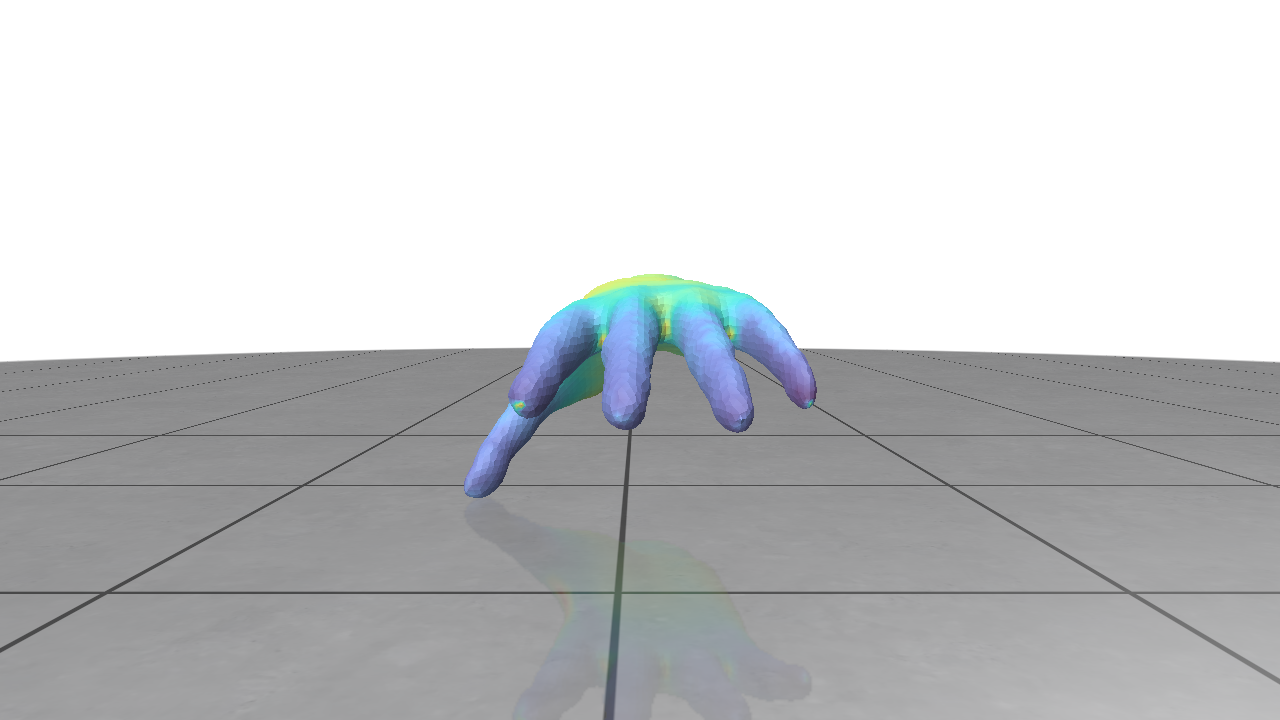
\includegraphics[width=0.65\textwidth]{../image/181_pymeshlab.png} \\
\cellcolor{blue!15}\textbf{Difference} \\
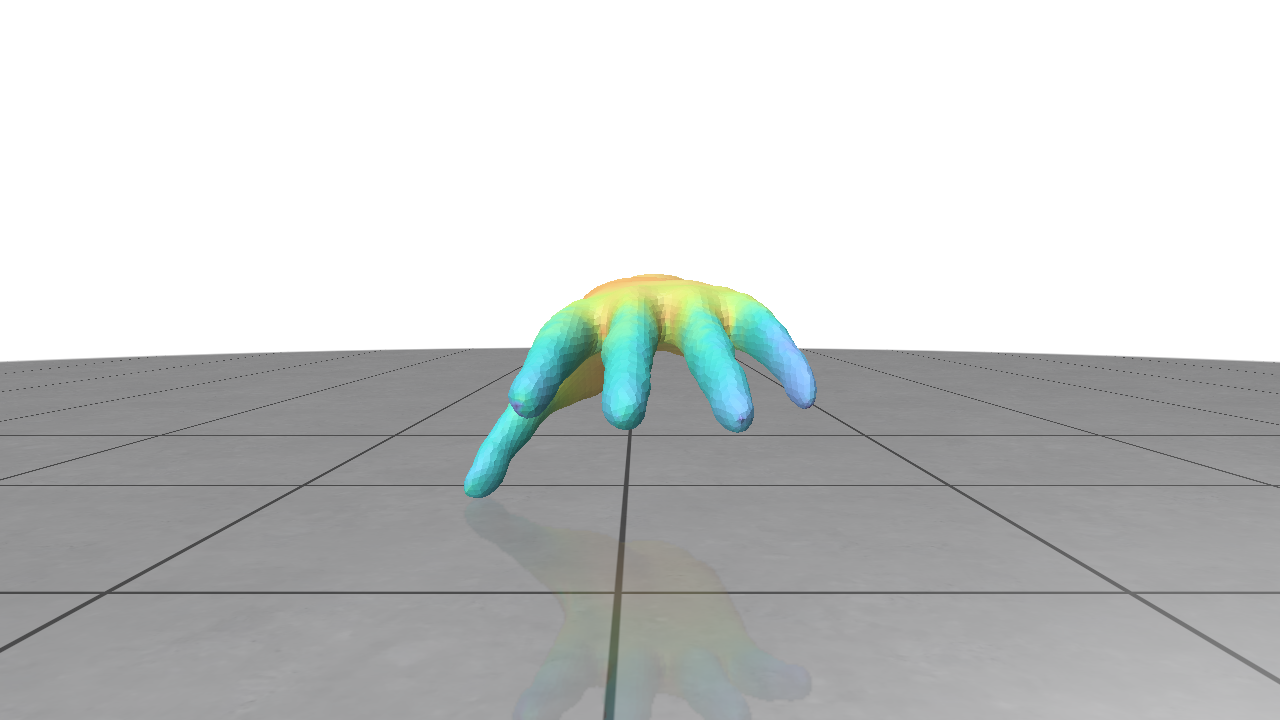
\includegraphics[width=0.65\textwidth]{../image/181_diff.png} \\
\end{tabular}
\caption{SDF quality comparison for model 181.obj (7,242 vertices)}
\label{fig:quality_181}
\end{figure}

Model 181 has 7,242 vertices and features a mix of smooth and sharp surface regions. The OptiX heat map captures smooth thickness gradients while preserving sharp transitions at feature edges. The PyMeshLab result shows comparable overall accuracy but with slightly more noise in flat regions. The difference map confirms that both implementations produce consistent SDF values, with the bilateral smoothing in OptiX contributing to a cleaner result.

\begin{figure}[ht]
\centering
\begin{tabular}{@{}c@{}}
\cellcolor{red!15}\textbf{OptiX} \\
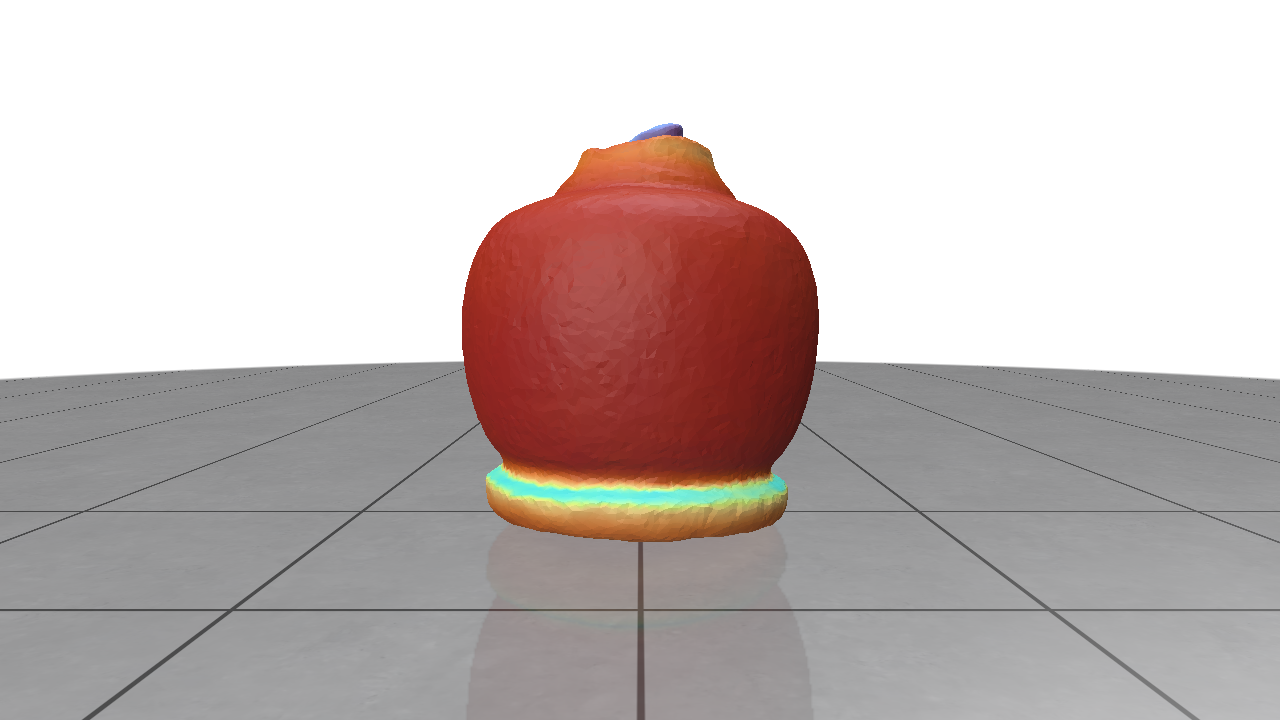
\includegraphics[width=0.65\textwidth]{../image/368_optix.png} \\
\cellcolor{green!15}\textbf{PyMeshLab} \\
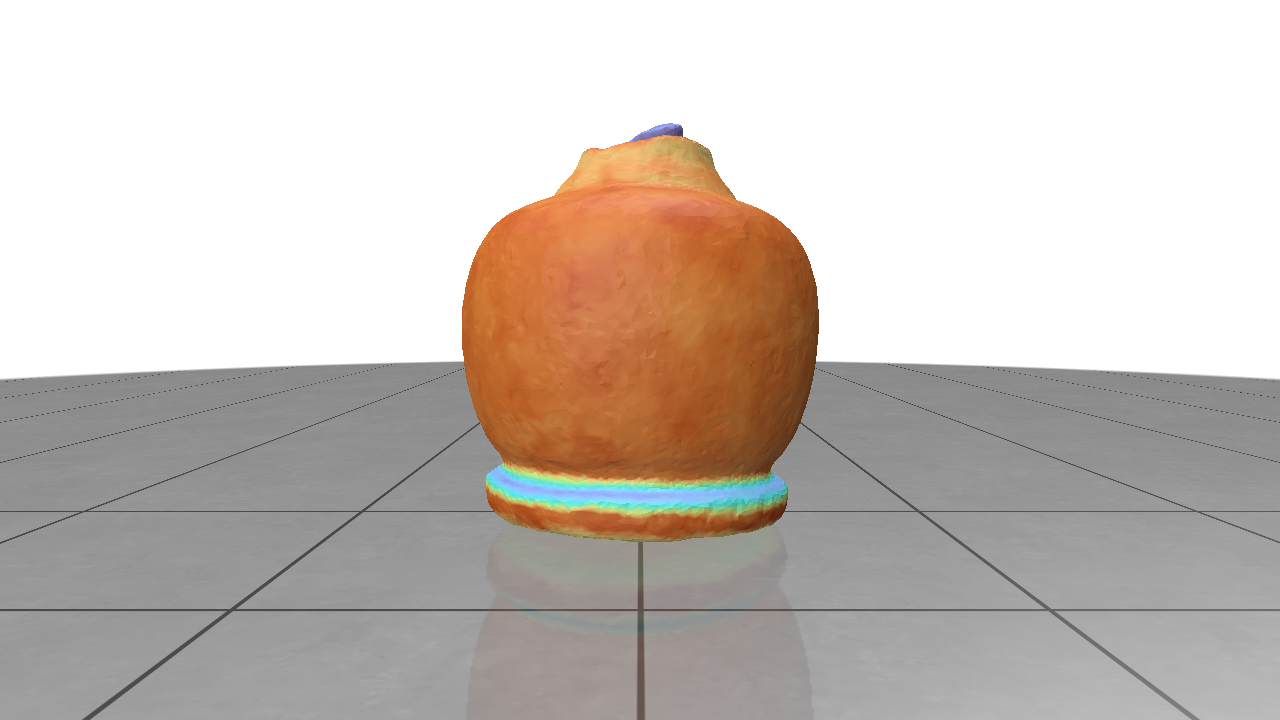
\includegraphics[width=0.65\textwidth]{../image/368_pymeshlab.png} \\
\cellcolor{blue!15}\textbf{Difference} \\
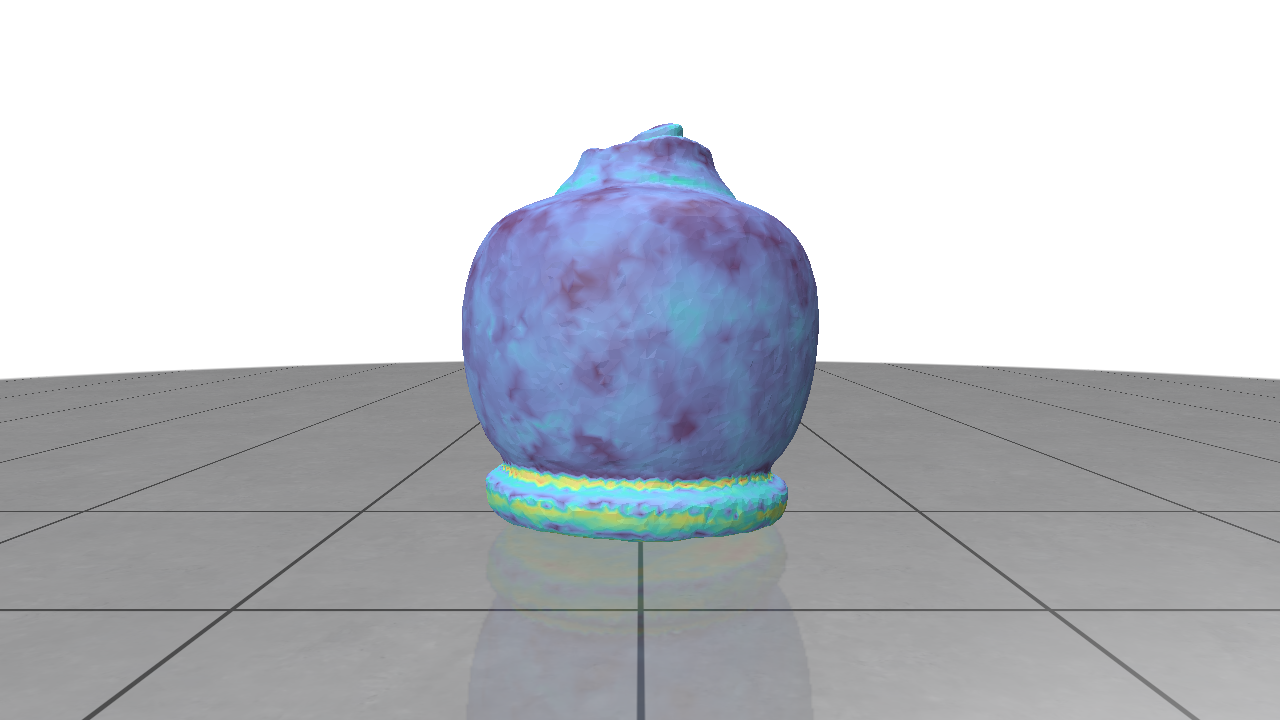
\includegraphics[width=0.65\textwidth]{../image/368_diff.png} \\
\end{tabular}
\caption{SDF quality comparison for model 368.obj (11,202 vertices)}
\label{fig:quality_368}
\end{figure}

Model 368 is a high-complexity model with 11,202 vertices. The OptiX pipeline produces a clean heat map where thick and thin regions are clearly distinguished. The PyMeshLab result shows slightly noisier transitions between regions of different thickness. The difference map reveals that the deviations are concentrated at boundary areas between thick and thin sections, where the bilateral smoothing filter in OptiX produces smoother gradients.

\begin{figure}[ht]
\centering
\begin{tabular}{@{}c@{}}
\cellcolor{red!15}\textbf{OptiX} \\
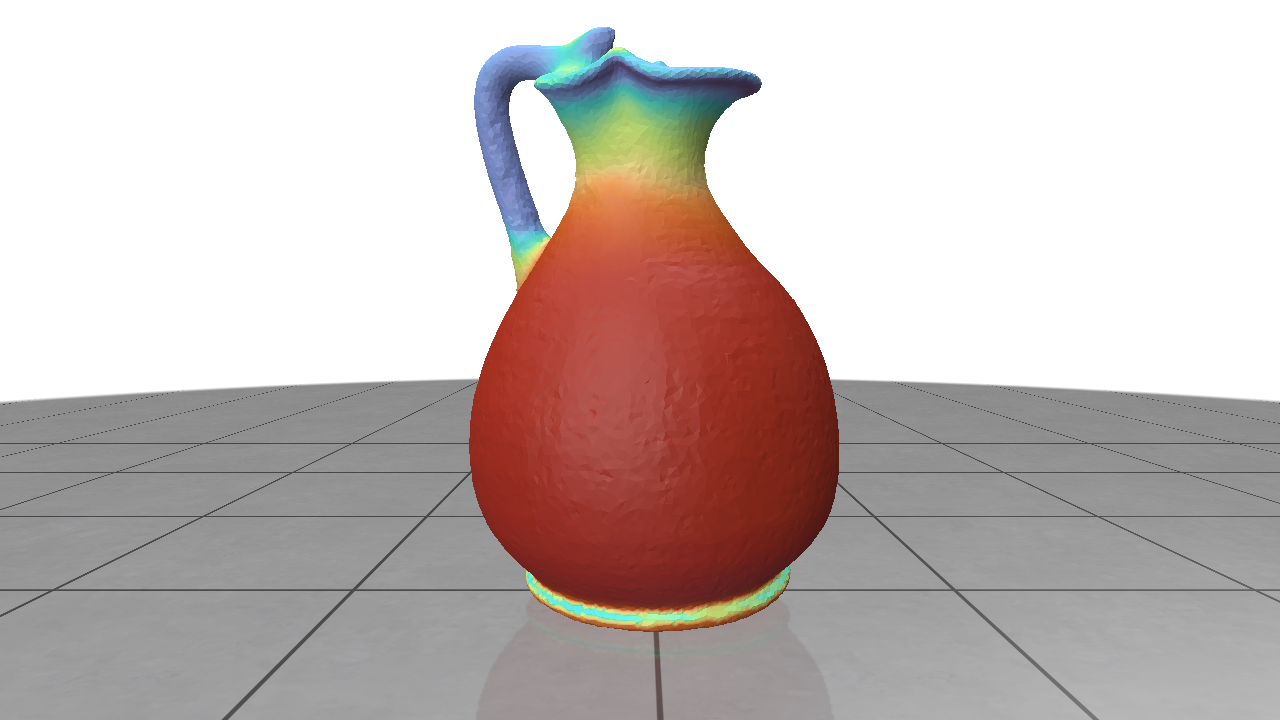
\includegraphics[width=0.65\textwidth]{../image/369_optix.png} \\
\cellcolor{green!15}\textbf{PyMeshLab} \\
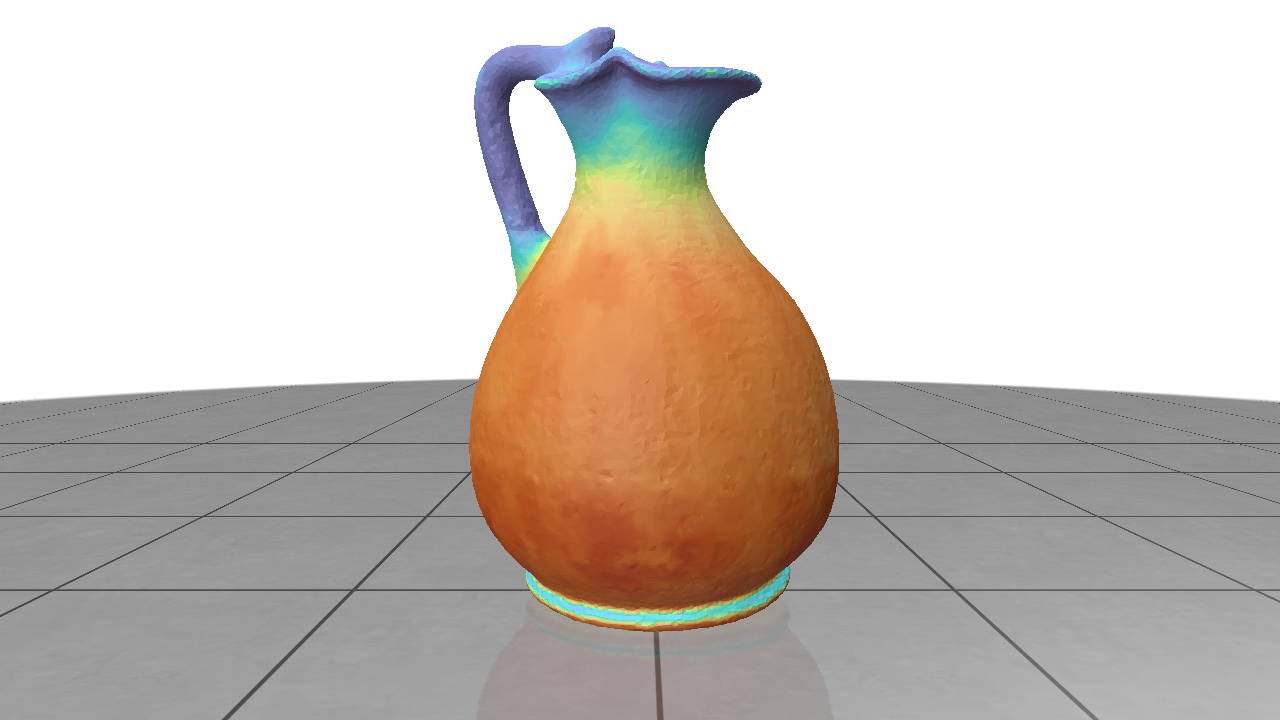
\includegraphics[width=0.65\textwidth]{../image/369_pymeshlab.png} \\
\cellcolor{blue!15}\textbf{Difference} \\
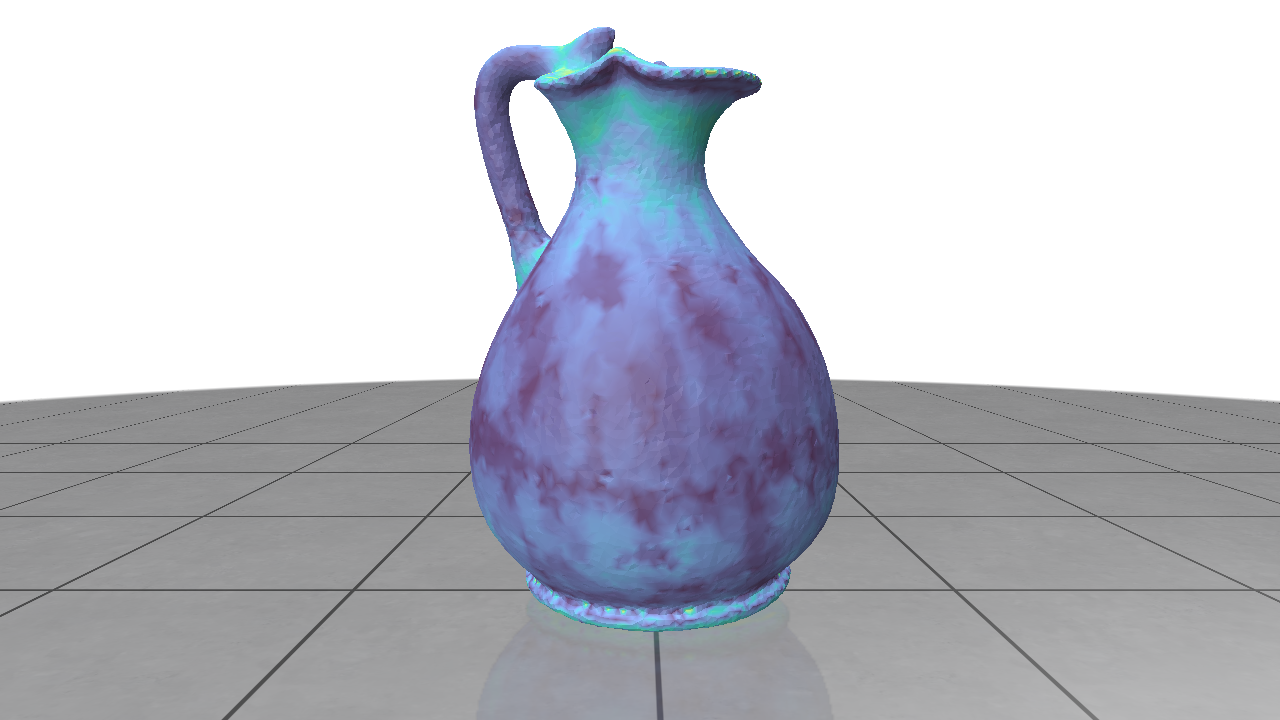
\includegraphics[width=0.65\textwidth]{../image/369_diff.png} \\
\end{tabular}
\caption{SDF quality comparison for model 369.obj (13,606 vertices)}
\label{fig:quality_369}
\end{figure}

Model 369 is comparable in size to model 112 with 13,606 vertices. The OptiX result shows well-preserved thickness features with smooth interpolation across flat surfaces. The PyMeshLab output captures the same overall structure but with more high-frequency noise. The difference map shows that both implementations produce consistent SDF values over large regions, with localized differences at fine geometric details.

\begin{figure}[ht]
\centering
\begin{tabular}{@{}c@{}}
\cellcolor{red!15}\textbf{OptiX} \\
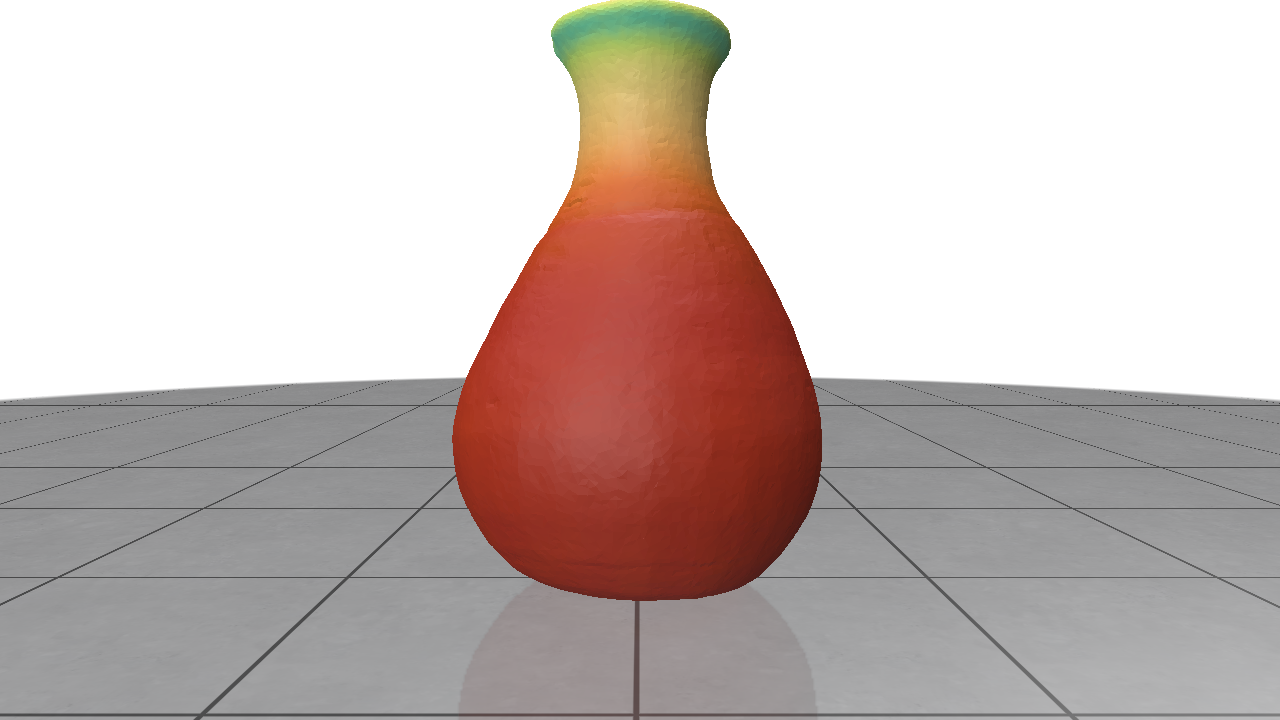
\includegraphics[width=0.65\textwidth]{../image/371_optix.png} \\
\cellcolor{green!15}\textbf{PyMeshLab} \\
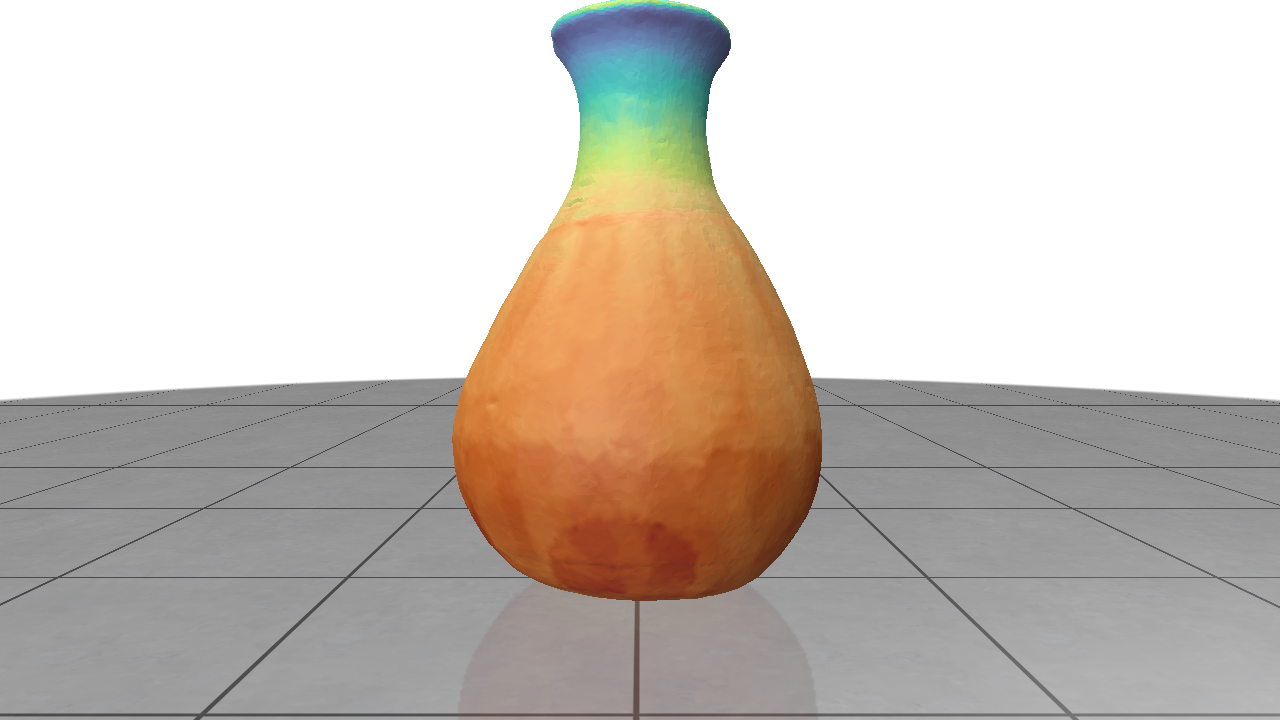
\includegraphics[width=0.65\textwidth]{../image/371_pymeshlab.png} \\
\cellcolor{blue!15}\textbf{Difference} \\
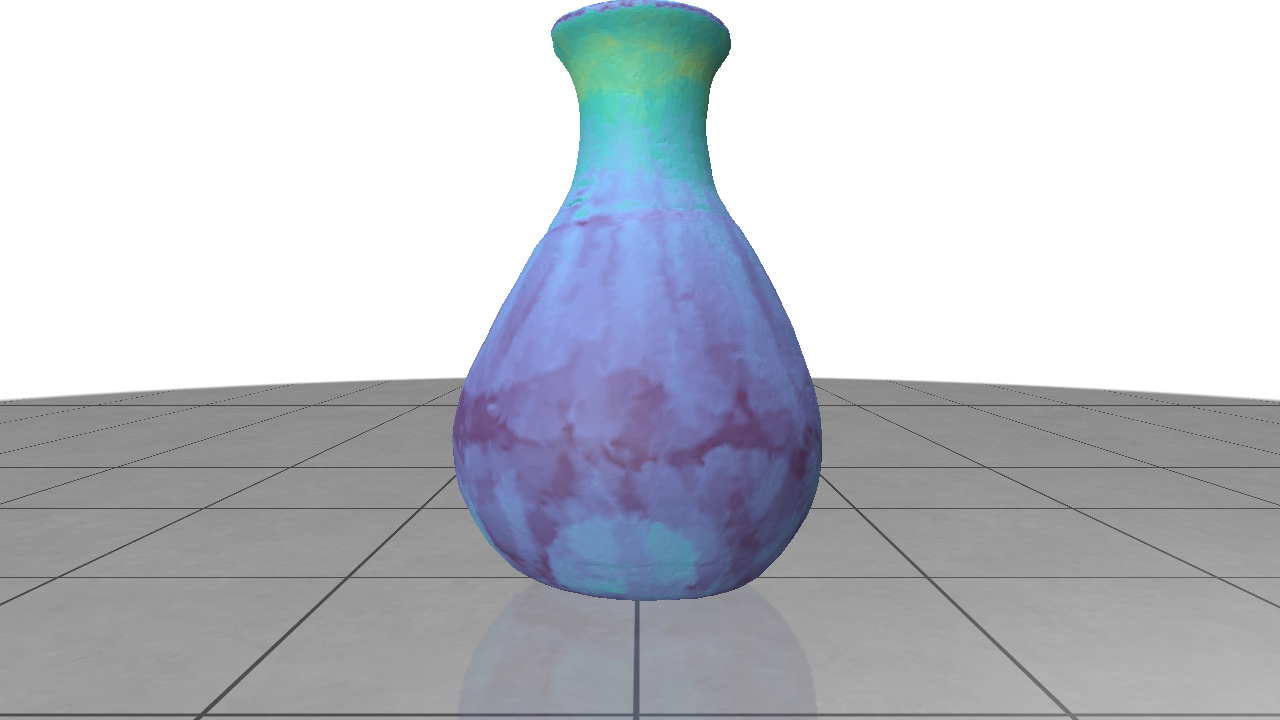
\includegraphics[width=0.65\textwidth]{../image/371_diff.png} \\
\end{tabular}
\caption{SDF quality comparison for model 371.obj (14,599 vertices)}
\label{fig:quality_371}
\end{figure}

Model 371 has the second-highest vertex count at 14,599. The OptiX heat map displays smooth, artifact-free thickness values across the entire surface. The PyMeshLab result is visually similar but exhibits minor noise in regions of uniform thickness. The difference map confirms that the two implementations produce closely matching results, with the bilateral smoothing in OptiX contributing to a cleaner output.

\begin{figure}[ht]
\centering
\begin{tabular}{@{}c@{}}
\cellcolor{red!15}\textbf{OptiX} \\
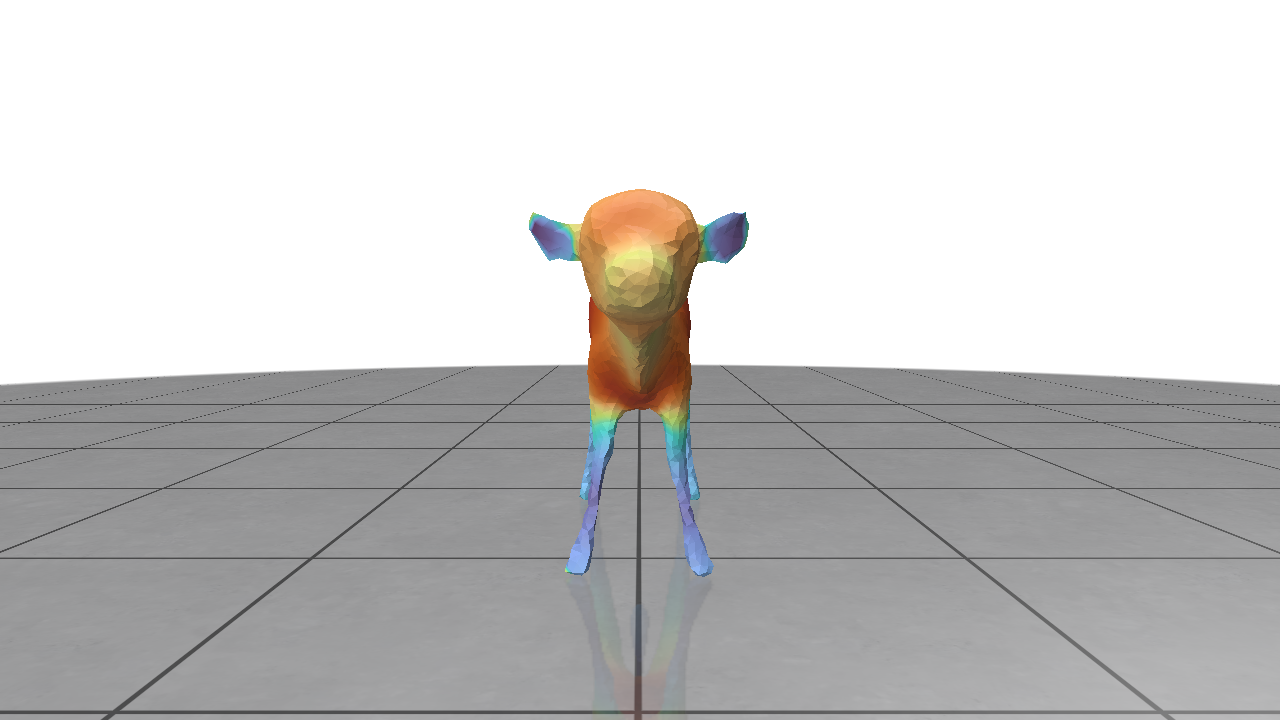
\includegraphics[width=0.65\textwidth]{../image/400_optix.png} \\
\cellcolor{green!15}\textbf{PyMeshLab} \\
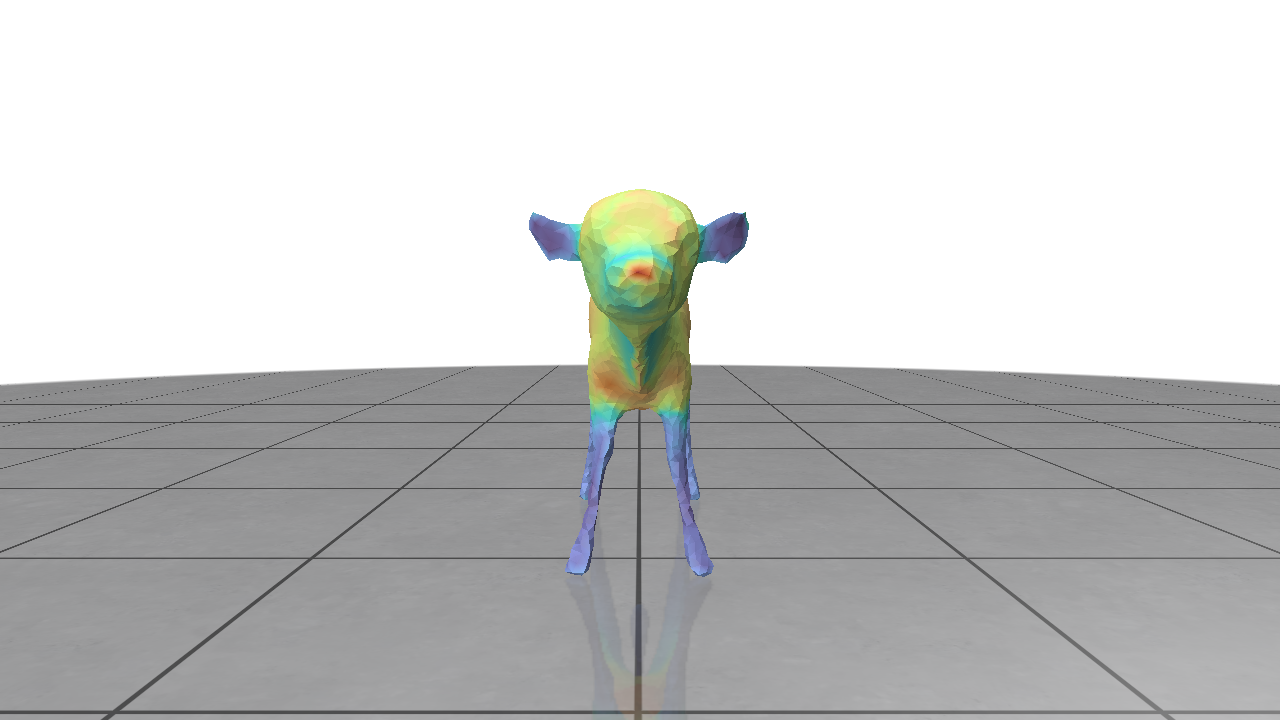
\includegraphics[width=0.65\textwidth]{../image/400_pymeshlab.png} \\
\cellcolor{blue!15}\textbf{Difference} \\
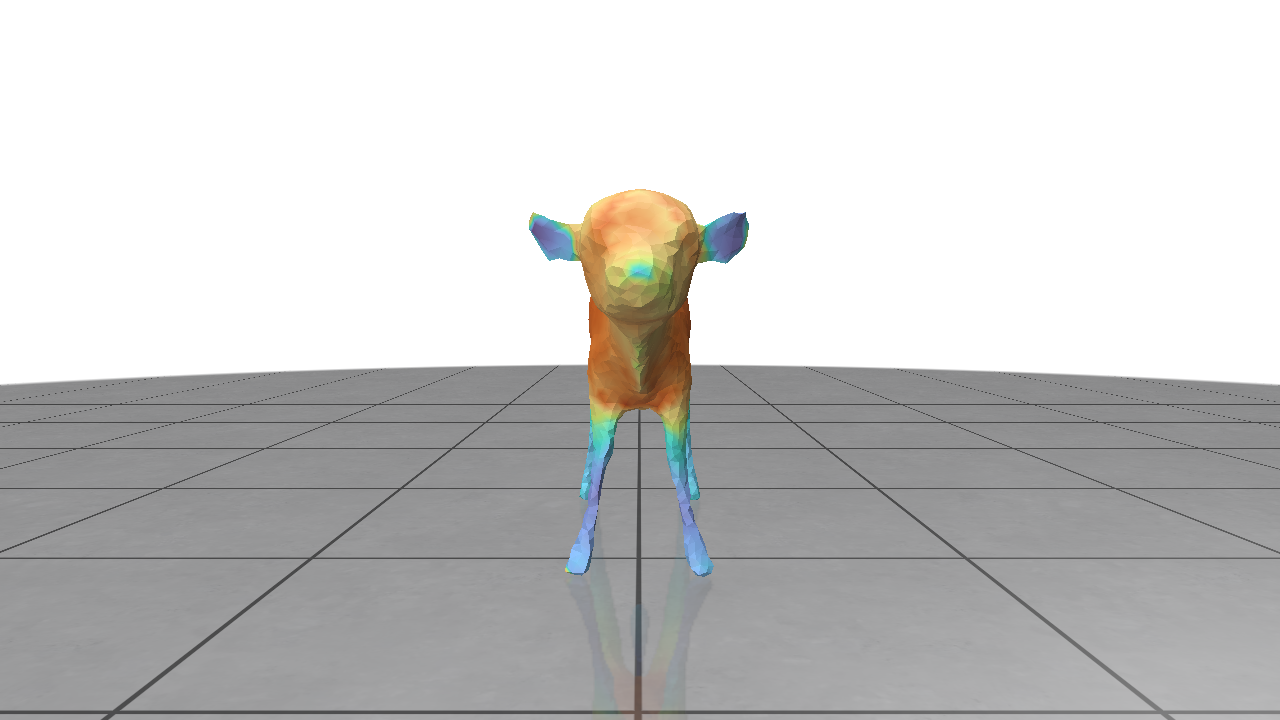
\includegraphics[width=0.65\textwidth]{../image/400_diff.png} \\
\end{tabular}
\caption{SDF quality comparison for model 400.obj (3,703 vertices)}
\label{fig:quality_400}
\end{figure}

Model 400 is a smaller model with 3,703 vertices. The OptiX heat map shows a clean, well-defined thickness distribution. The PyMeshLab result is nearly identical, with only subtle differences visible in the difference map. For small models, both implementations produce highly consistent SDF values, and the performance advantage of OptiX (33.2x speedup) does not come at the cost of quality.

\begin{figure}[ht]
\centering
\begin{tabular}{@{}c@{}}
\cellcolor{red!15}\textbf{OptiX} \\
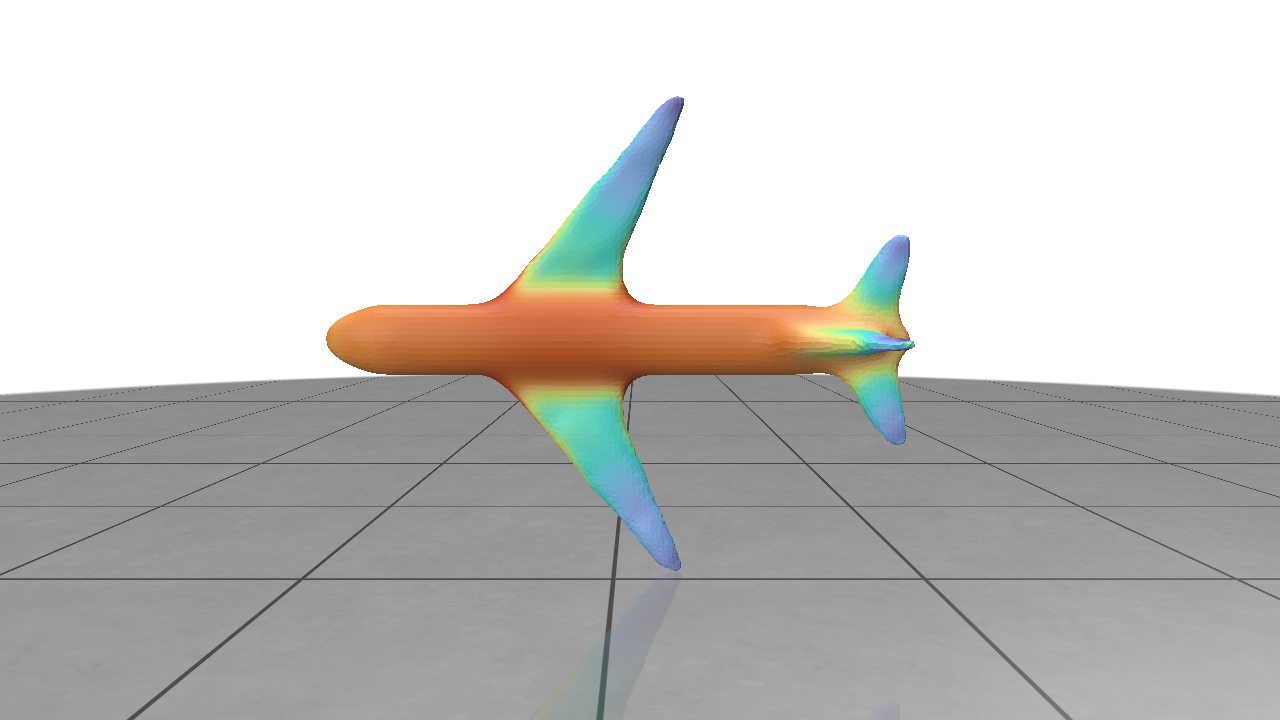
\includegraphics[width=0.65\textwidth]{../image/76_optix.png} \\
\cellcolor{green!15}\textbf{PyMeshLab} \\
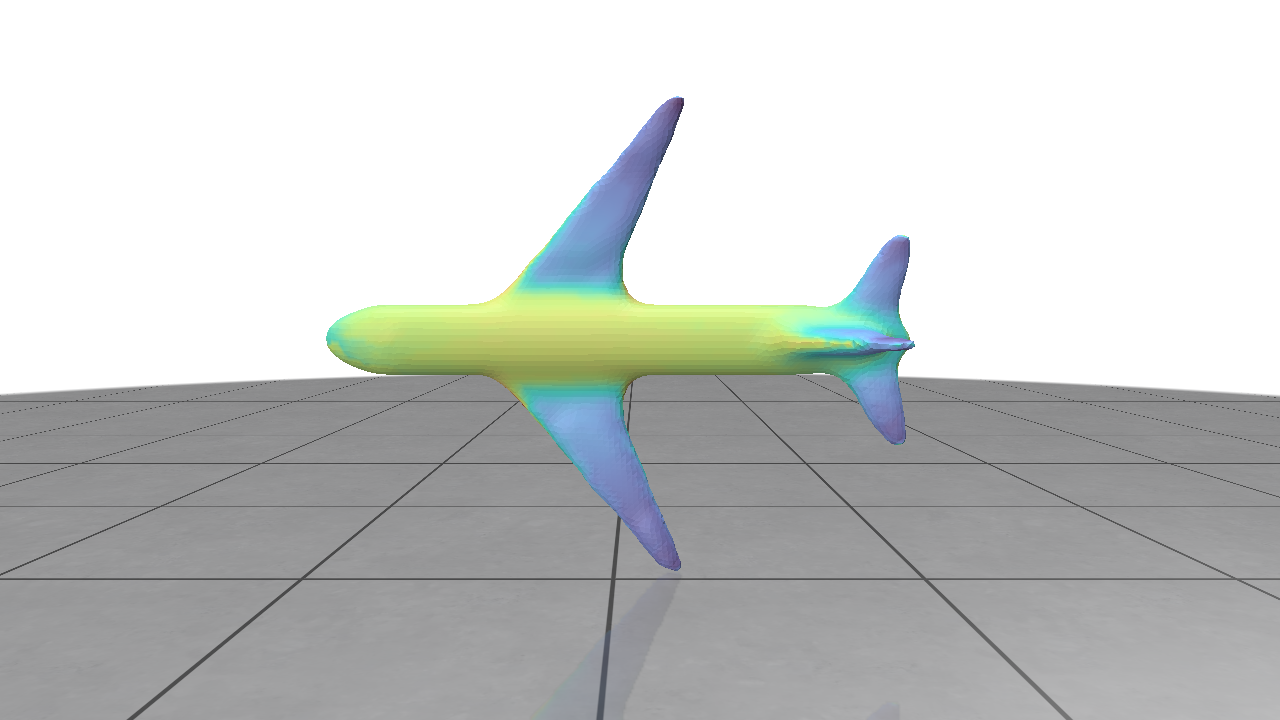
\includegraphics[width=0.65\textwidth]{../image/76_pymeshlab.png} \\
\cellcolor{blue!15}\textbf{Difference} \\
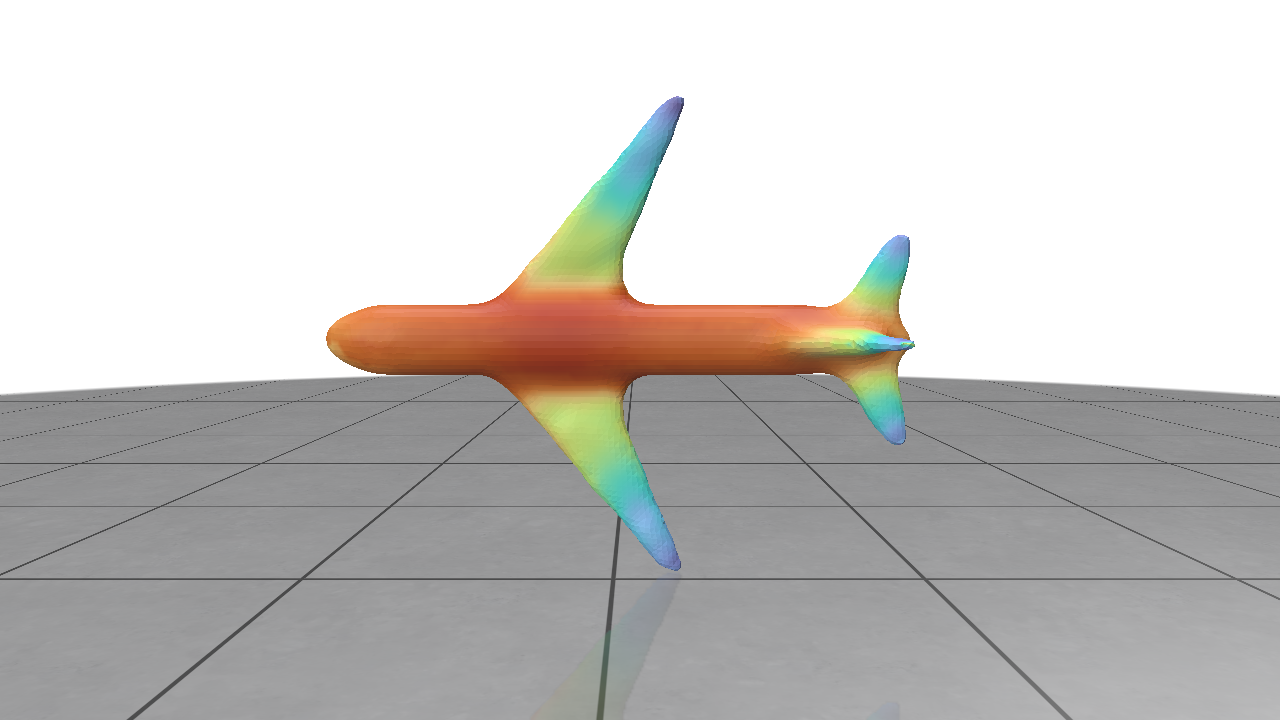
\includegraphics[width=0.65\textwidth]{../image/76_diff.png} \\
\end{tabular}
\caption{SDF quality comparison for model 76.obj (5,923 vertices)}
\label{fig:quality_76}
\end{figure}

Model 76 is a medium-complexity model with 5,923 vertices. The OptiX result shows smooth thickness transitions across the surface, while the PyMeshLab result exhibits minor noise in regions of gradual thickness change. The difference map shows that the largest deviations occur at edges and thin features, where the bilateral smoothing filter in OptiX better preserves sharp boundaries.

\begin{figure}[ht]
\centering
\begin{tabular}{@{}c@{}}
\cellcolor{red!15}\textbf{OptiX} \\
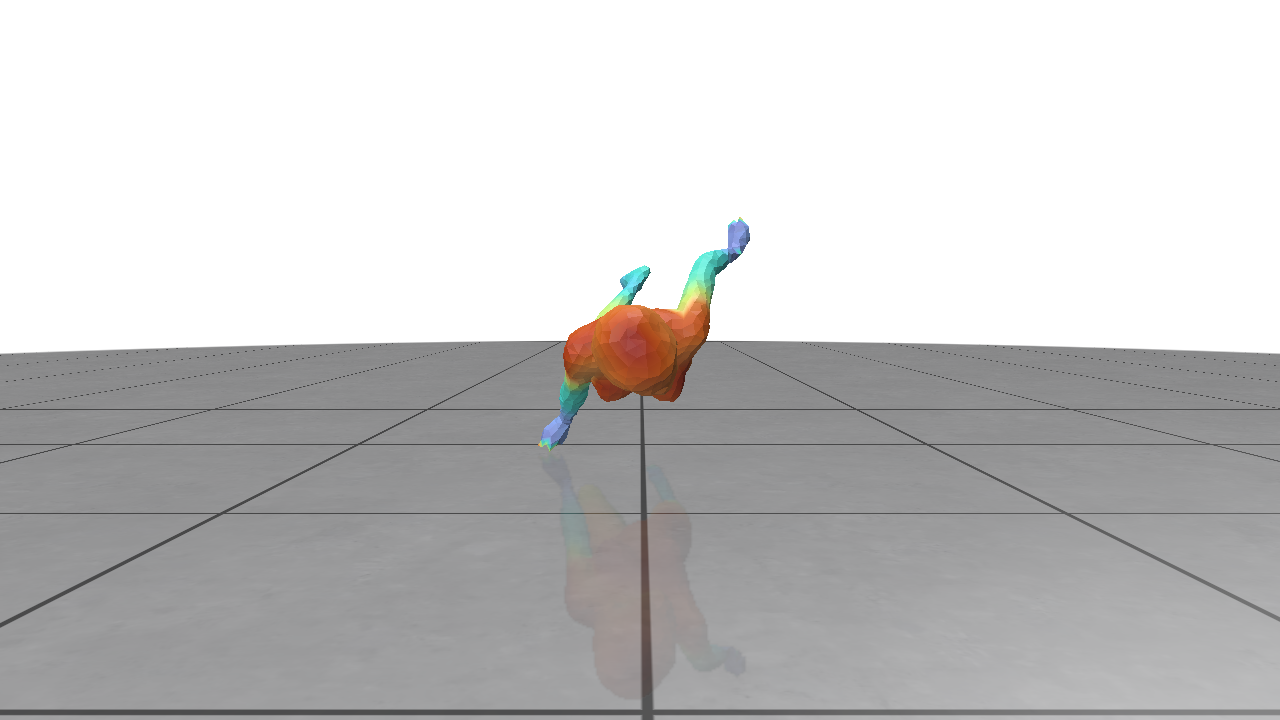
\includegraphics[width=0.65\textwidth]{../image/9_optix.png} \\
\cellcolor{green!15}\textbf{PyMeshLab} \\
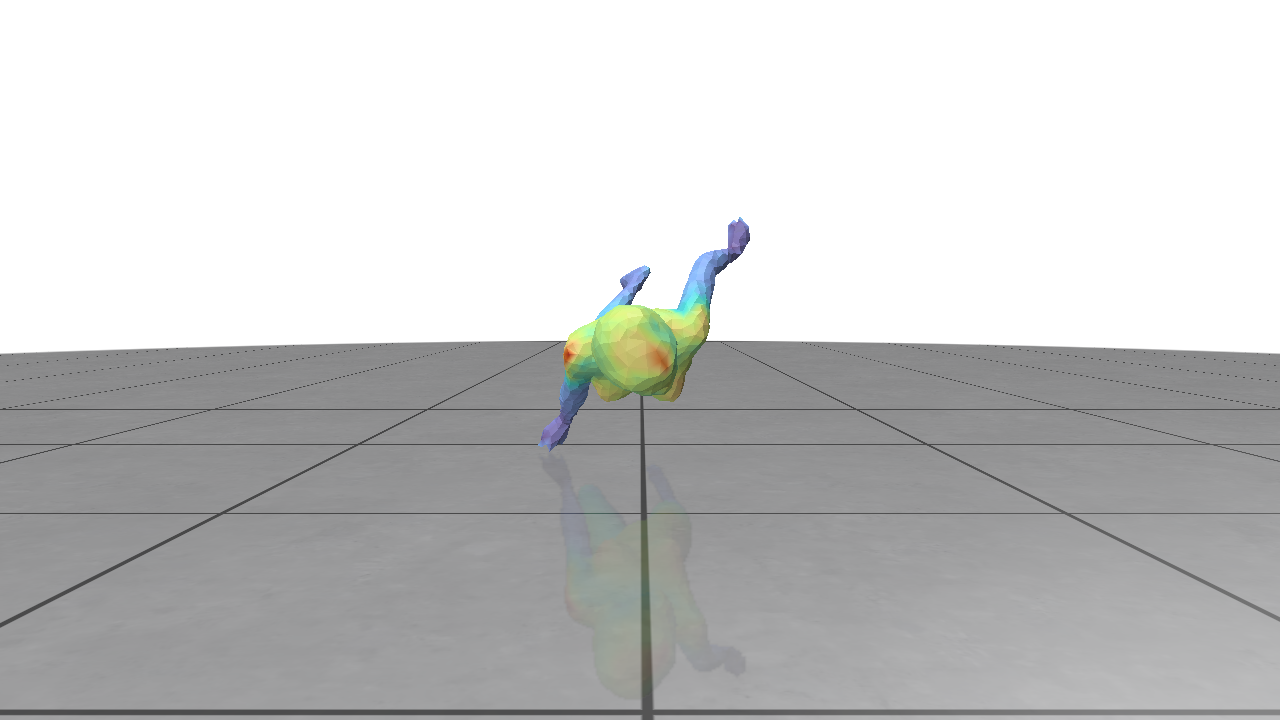
\includegraphics[width=0.65\textwidth]{../image/9_pymeshlab.png} \\
\cellcolor{blue!15}\textbf{Difference} \\
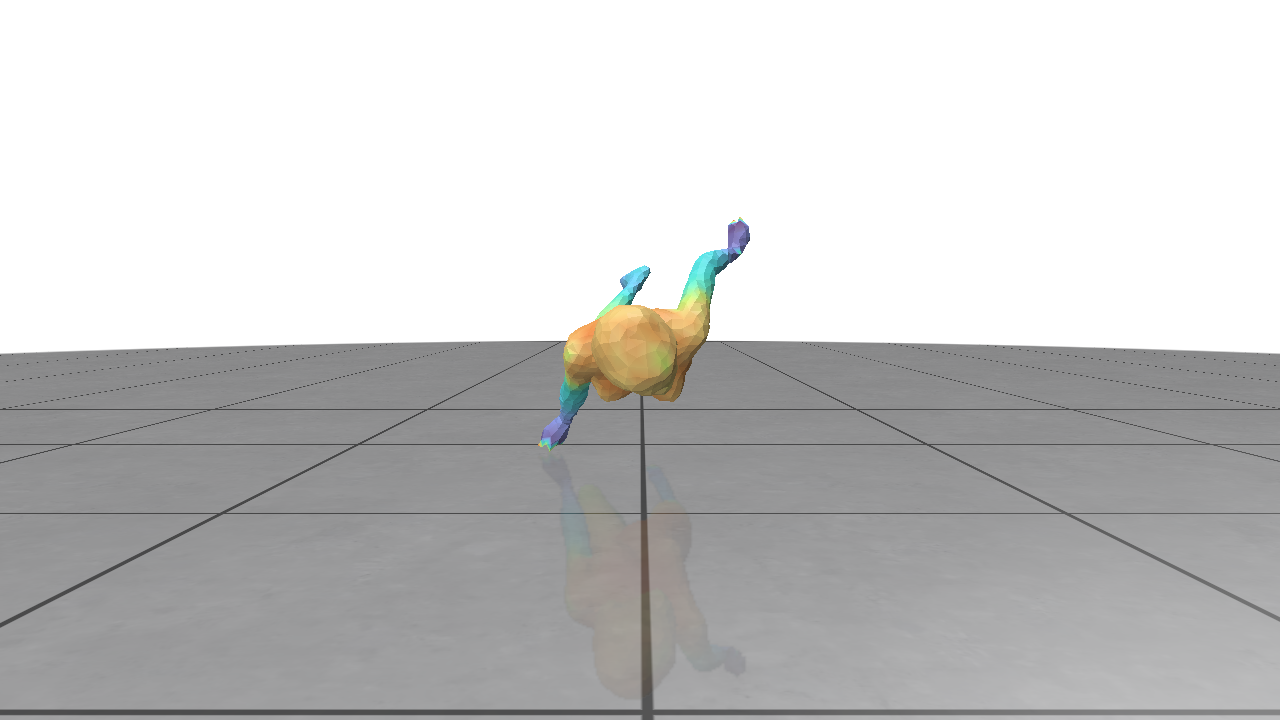
\includegraphics[width=0.65\textwidth]{../image/9_diff.png} \\
\end{tabular}
\caption{SDF quality comparison for model 9.obj (2,639 vertices)}
\label{fig:quality_9}
\end{figure}

Model 9 is the second-smallest model with only 2,639 vertices. Both implementations produce visually similar heat maps with consistent thickness values. The difference map shows minimal discrepancy, confirming that the OptiX pipeline maintains quality even for small, simple meshes. The 51.6x speedup demonstrates that OptiX provides significant performance gains across all model scales.

\clearpage

\section{Overall Conclusion}

Despite the huge difference in computation time (3.1x to 171x speedup), the OptiX SDF is still smoother than the PyMeshLab result. This is because the OptiX pipeline includes anisotropic bilateral smoothing as a post-processing step, which reduces noise while preserving sharp features. The PyMeshLab implementation produces raw SDF values without any smoothing, resulting in noisier outputs. The OptiX approach demonstrates that hardware ray tracing can simultaneously improve both performance and quality for geometric analysis tasks.


% =========================================================================
% REFERENCES
% =========================================================================
\newpage
\addcontentsline{toc}{chapter}{References}
\begin{thebibliography}{9}

\bibitem{shapira2008}
L. Shapira, A. Shamir, D. Cohen-Or,
\newblock ``Consistent Mesh Partitioning and Skeletonization using the Shape Diameter Function,''
\newblock \emph{Visual Computer}, vol.~24, pp.~249--259, 2008.

\bibitem{kamenicky2014}
J. Kamenick\'{y},
\newblock ``Parallelization of Shape Diameter Function Computation using OpenCL,''
\newblock \emph{Proceedings of CESCG}, 204, 2014.

\bibitem{chen2018}
S. Chen, T. Liu, Z. Shu, S. Xin, Y. He, C. Tu,
\newblock ``Fast and robust shape diameter function,''
\newblock \emph{PLoS ONE}, vol.~13, no.~1, e0190666, 2018.

\bibitem{vcglib}
VCG Library,
\newblock ``Visualization and Computer Graphics Library,''
\newblock \url{https://github.com/cnr-isti-vclab/vcglib}.

\bibitem{optix}
NVIDIA Corporation,
\newblock ``NVIDIA OptiX Ray Tracing Engine,''
\newblock \url{https://developer.nvidia.com/optix}.

\bibitem{cuda}
NVIDIA Corporation,
\newblock ``CUDA C Programming Guide,''
\newblock \url{https://docs.nvidia.com/cuda/cuda-c-programming-guide/}.

\end{thebibliography}

\end{document}
